\documentclass{article}
\usepackage{ctex}
\usepackage[utf8]{inputenc}
%\usepackage{natbib}
\usepackage[square,sort,comma,numbers]{natbib}
\usepackage{graphicx}
\usepackage{geometry}
\usepackage{booktabs}
\usepackage{siunitx}
\usepackage{listings}
\usepackage{subfigure}
\usepackage{appendix}
\usepackage{graphicx}
\usepackage{pythonhighlight}
\usepackage{setspace}
\lstset{numbers=left, %设置行号位置
        numberstyle=\tiny, %设置行号大小
        keywordstyle=\color{blue}, %设置关键字颜色
        commentstyle=\color[cmyk]{1,0,1,0}, %设置注释颜色
        frame=single, %设置边框格式
        %escapeinside=, %逃逸字符(1左面的键),用于显示中文
        breaklines, %自动折行
        extendedchars=false, %解决代码跨页时,章节标题,页眉等汉字不显示的问题
        xleftmargin=2em,xrightmargin=2em, aboveskip=1em, %设置边距
        tabsize=4, %设置tab空格数
        showspaces=false %不显示空格
}
\usepackage{arydshln}
\usepackage{listings} % code display
\geometry{a4paper,centering,scale=0.8}
\usepackage[format=hang,font=small,textfont=it]{caption}
\usepackage[nottoc]{tocbibind}
\usepackage{float}
\usepackage{amsmath}
\usepackage[colorlinks=true, 
    linkcolor=blue,          % color of internal links
    citecolor=blue,        % color of links to bibliography
    filecolor=blue,      % color of file links
    urlcolor=blue]{hyperref}
    \usepackage[myheadings]{fullpage}
\numberwithin{equation}{subsection}
\newcommand{\HRule}[1]{\rule{\linewidth}{#1}}
\newcommand\degree{^\circ}
\date{}
%\bibliographystyle{plain}
\usepackage{abstract}
\setlength{\abstitleskip}{0em}%“摘要”与摘要正文间距
\renewcommand{\abstractnamefont}{\Large\bfseries}
\pagestyle{plain}
\geometry{a4paper,left=3cm,right=3cm}

%=================================================================================================================
\title{\heiti 基于分类模型的慢性病相关因素研究}
%这里填写题目
\begin{document}
\maketitle

\vspace{-5em}%“摘要”与标题的间距
\begin{abstract}
以心脑血管疾病、糖尿病、恶性肿瘤以及慢性阻塞性肺病为代表的慢性非传染性疾病(以下
简称慢性病)已经成为影响我国居民身体健康的重要问题。随着人们生活方式的改变,慢性病的患病率持续攀升。众所周知,健康状况与年龄、饮食习惯、身体活动情况、职业等都有密切的关系。如何通过合理地安排膳食、适量的身体运动、践行健康的生活方式,从而达到促进身体健康的目的,这是全社会普遍关注的问题。

\textbf{针对问题一:}通过中国营养学会最新修订的《中国居民膳食指南》中为平衡居民膳食提出的八条准则,利用附件A2的调查数据,我们对数据进行整合计算,得到例如每人每日谷薯类食物摄入量、BMI等新指标,设立对应标准以评判居民在食物多样性、吃动平衡性、多吃蔬果奶类等饮食习惯上的合理性。
%问题一摘要(\textbf{}加粗关键词)

\textbf{针对问题二:}在附件A2以及第一问设立的新指标的基础上,我们建立GUIDE决策树模型,分别寻找年龄、性别、文化程度、婚姻状况、职业与生活习惯、饮食习惯之间的关联,并通过重要性评分,来探寻不同的生活、饮食习惯对年龄、性别、文化程度、婚姻状况、职业相关性程度。
%问题二摘要(\textbf{}加粗关键词)

\textbf{针对问题三:}按照世界卫生组织给出的慢性病判断标准,我们给人群设定是否得高血压、是否得糖尿病、是否得高血脂、是否得高尿酸血症这四种慢性病指标。在附件A2以及第一问设立的新指标的基础上,结合上述慢性病指标,我们建立二分类Logistic回归模型,根据“奥卡姆剃刀”原理进行两次回归处理和显著性p值检验,得到了关于高血压、糖尿病、高血脂、高尿酸血脂和吸烟、饮酒、饮食习惯、工作状况、运动强度等因素之间的联系。
%问题三摘要(\textbf{}加粗关键词)

\textbf{针对问题四:}在问题一与问题三建立的模型基础上,我们将居民划分为四大类。即慢性病患者、潜在慢性病患者、习惯不合理的健康居民以及习惯合理的健康居民。我们通过每一类人群与其对应模型中的强相关因素,给每一类人群给出适当的饮食、生活上的建议。
%问题四摘要(\textbf{}加粗关键词)

\textbf{关键词:慢性病;决策树;Logistic回归}
\end{abstract}
\newpage

%============================================================================================================
{\centering\section{问题重述}}
近年来,随着人们生活方式的改变,我国居民慢性病的患病率持续攀升,以心脑血管疾病、糖尿病、恶性肿瘤以及慢性阻塞性肺病为代表的慢性非传染性疾病已经成为影响我国居民身体健康的重要问题。
为了研究年龄、饮食习惯、身体活动情况、职业等因素对健康状况的影响关系,某市卫生健康研究部门对部分居民进行了问卷调查。相应的问卷表及调查结果如附件所示。
请参考《中国居民膳食指南》中提出的平衡膳食的八条准测,探究并解决以下问题:

\textbf{问题1:}参考附件A3,分析附件A2中居民的饮食习惯的合理性并说明存在的主要问题。

\textbf{问题2:}根据附件A2中的数据,分析居民的生活习惯和饮食习惯是否与年龄、性别、婚姻状况、文化程度、职业等因素相关。

\textbf{问题3:}根据附件A2中的数据,深入分析常见慢性病(如高血压、糖尿病等)与吸烟、饮酒、饮食习惯、生活习惯、工作性质、运动等因素的关系以及相关程度。

\textbf{问题4:}依据附件A2中居民的具体情况,对居民进行合理分类,并针对各类人群提出有利于身体健康的膳食、运动等方面的合理建议。
%============================================================================================================
\vskip 0.5cm
{\centering\section{问题分析与数据处理}}

\subsection{数据预处理}
附件A2中的数据存在以下缺陷不便于分析,先进行数据预处理如下:

\textbf{缺陷1:}附件A2数据表存在较多空行,部分数据无ID序号,影响数据导入程序。

\textbf{解决1:}手动删除空行并重新编号。

\textbf{缺陷2:}饮酒情况与饮食情况的用量数据单位不统一,不便与平衡膳食的八条准则比对。

\textbf{解决2:}统一用量单位为“克每人每日”,具体量器单位换算参考附件A1。

预处理后的数据表详见附件“数据处理.xlsx”。进行了行位置调整的数据ID用红色标记,用量单位换算后得到的数据用黄色列展示。
%-------------------------------------------------
\subsection{问题一的分析与数据处理}

题目要求分析居民饮食习惯的合理性,只需关注饮酒情况与饮食情况的调查数据。对于八条准则中要求控制摄入量的膳食,如果其在问卷中仅对应一种食物(例如:每天摄入不少于300g的新鲜蔬菜,“新鲜蔬菜”膳食仅对应问卷中“新鲜蔬菜 ”这一种食物),则以该食物的摄入量作为该膳食的摄入量;如果该膳食对应问卷中的多种食物(例如:每天摄入约120-200g的鱼禽、蛋类和瘦肉,“鱼禽、蛋类和瘦肉”膳食对应问卷中的“猪肉、牛羊肉、禽肉、水产品、蛋类”五种食物),则以多种对应食物的摄入量之和作为该膳食的摄入量。

经过上述处理可得每种膳食不同人的日摄入量。继而绘制散点图,对同种膳食每人的日摄入量求平均值并与八条准则中的标准值相比较,从而分析居民饮食习惯中的问题及八条准则的合理性。

%--------------------------------------------------
\subsection{问题二的分析与数据处理}
问题二探究的是单一离散变量(如年龄,婚姻状况)不同种类关于多变量(生活、饮食习惯)之间的特征关系,考虑到决策树分类器对自变量因素的选择能力和特点,决定采用GUIDE决策树模型,通过考虑不同变量对因变量种类分类的差异性能力来进行重要性评分,来得到分类模型与不同人群的特征。

由于生活、饮食习惯中的因素往往相互关联互相作用,除问卷中调查的各项指标外,我们也参考了相关资料 \cite {1},将某些指标合并作为新的因子,整理得到“生活、饮食习惯”的参考指标(详见附件“变量说明.xlsx”)。

%--------------------------------------------------
\subsection{问题三的分析与数据处理}
从体检指标入手,根据世界卫生组织给出的慢性病评价标准,为居民们标注是否高血压、是否糖尿病、是否高血脂、是否高尿酸血症这四种慢性病指标。由于这些慢性病指标为0-1的二分类指标,考虑分别对其使用Logistic回归模型,自变量为吸烟、饮酒、饮食习惯、工作状况、运动等指标。

由于自变量维度过高,对每个自变量使用显著性p值检验,p值高于0.05的自变量即为在模型中表现不显著,去除;p值低于0.05的自变量即为在模型中表现显著,保留。根据奥卡姆剃刀原理,利用留下的有显著影响的自变量再进行一次Logistic回归,得到各慢性病与生活习惯饮食习惯之间的关系。

%--------------------------------------------------
\subsection{问题四的分析与数据处理}
根据问题一与问题三给出的分类模型,我们尝试对居民的健康状况进行分类。利用问题三中给出的慢性病评价标准,我们将人群分出慢性病患者;利用问题三中的慢性病预测模型,我们将非患者人群中分出潜在慢性病患者;利用问题一给出的生活饮食习惯评价指标,分出了习惯不合理的健康人群以及习惯合理的健康人群。依据问题三中给出的慢性病预测模型和相关因素,我们给慢性病患者和潜在慢性病患者给出合适的膳食运动建议;依据问题一给出的习惯评价指标,为习惯不合理的健康人群给出合适的膳食运动建议。

%============================================================================================================
{\centering\section{模型假设}}

\textbf{假设一:}问卷调查时间为2023年。

\noindent
分析居民的生活习惯时,年龄、烟龄是重要的指标,但问卷中并未明确。鉴于最新版《中国居民膳食指南》出版时间为2022年,假设问卷调查时间为2023年,即居民的年龄、烟龄为2023年的年龄、烟龄。
    
\textbf{假设二:}啤酒5°,葡萄酒12°,黄酒15°,低度白酒35°,高度白酒50°。

\noindent
平衡膳食的八条准则中对每日摄入酒精含量做出了明确规定,但问卷中并未明确酒精含量。经充分考察资料\cite {2} ,假设问卷中的酒精含量为上述值。

\textbf{假设三:}主要成分相同的食物具有可加性(酒精参考假设2)。

\noindent
由于问卷中的食物种类较多,且每种食物的成分不同,为了方便计算,假设主要成分相同的食物具有可加性,即每种食物的主要成分之和为该食物的总成分。(例如:奶制品摄入量 = 牛奶摄入量 + 酸奶摄入量 + 奶酪摄入量)

\textbf{假设四:}奶制品的标准摄入量为200-500g/人/日

\noindent
附件A3仅给出了奶制品的最高摄入量而无最低摄入量,显然不够科学。经充分查阅相关资料\cite {1} ,假设奶制品的标准摄入量为200-500g/人/日。

%奶,300g标准引用%http://dg.cnsoc.org/article/04/RMAbPdrjQ6CGWTwmo62hQg.html


%============================================================================================================
{\centering\section{问题一的建模与求解}}

\subsection{模型建立}
根据八条准则提出的膳食标准是否精确到克数,分为定量型标准和非定量型标准。

\subsubsection{定量型膳食标准}
定量型标准(克每人每日)包含以下内容:

\begin{table}[H]
    \centering
    \setlength{\tabcolsep}{4mm}{ %调整表格横向宽度
    \begin{tabular}{cccc}
        \toprule[1.5pt]%调节横线1粗细
        膳食名称&	          对应食物的问卷编号	& 标准摄入量(克每人每日)	\\
    \midrule[1pt]%调节横线2粗细
        新鲜蔬菜	&	  D22 &		$\geq$ 300g \\
        新鲜水果	&	  D28 &		200-350g 		 \\
        奶制品 &		  D14,D15,D16 &		200-500g   \\
        烹调油	&	      D31,D32 &		25-30g  \\
        食用盐&		      D33 	&	<5g   \\
        酒精	&	   C3,C4,C5,C6,C7    &		<15g	  \\
        鱼禽蛋瘦肉&	D9,D10,D11,D13,D17 &	120-200g    \\
        \bottomrule[1.5pt]%调节横线3粗细
    \end{tabular}}
    \caption{平衡膳食八准则之定量型标准\\(注:根据假设3.5,奶制品的标准摄入量200-500g)}
\end{table}

根据问题分析2.2中提出的膳食摄入量计算方法,计算调查群体中每人每日的各膳食摄入量(见附件"问题1-1摄入量数据计算.xlsx")并绘制频率分布直方图(见附录1)。
注意:根据假设3.4,奶制品、烹调油、鱼禽蛋瘦肉这三类膳食得摄入量计算公式为(克每人每日):

\begin{equation}
    \left\{\begin{array}{l}
        \text{奶制品摄入量} = \text{牛奶摄入量} + \text{酸奶摄入量} + \text{奶酪摄入量} \\
        \text{烹调油摄入量} = \text{植物油摄入量} + \text{动物油摄入量} \\
        \text{鱼禽蛋瘦肉摄入量} = \text{猪肉摄入量} + \text{牛羊肉摄入量} + \text{禽肉摄入量} + \text{水产品摄入量} + \text{蛋类摄入量}\\
    \end{array}\right.
\end{equation}

根据假设3.2,酒精摄入量的计算公式为(克每人每日):

\begin{equation}
    \begin{aligned}
        \text{酒精摄入量}
        &=5\%*\text{啤酒摄入量}+12\%*\text{葡萄酒摄入量}+15\%*\text{黄酒摄入量}\\
        &+35\%*\text{低度白酒摄入量}+50\%*\text{高度白酒摄入量} \\
    \end{aligned}
\end{equation}

各膳食经运算后得到数据如下表所示:
\begin{table}[H]
    \centering
    \setlength{\tabcolsep}{3.5mm}{ %调整表格横向宽度
    \begin{tabular}{cccc}
        \toprule[1.5pt]%调节横线1粗细
        膳食名称&	          平均摄入量(克每人每日)	& 标准摄入量(克每人每日)&达标百分比	\\
    \midrule[1pt]%调节横线2粗细
        新鲜蔬菜	&	289.67g  &		$\geq$ 300g &51.82\%\\
        新鲜水果	&	  151.05g &		200-350g &		21.12\%\\
        奶制品 &		  93.64g &		200-500g &  13.97\%\\
        烹调油	&	      46.65g &		25-30g & 11.74\%\\
        食用盐&		 5.77g     	&	<5g  & 51.71\%\\
        酒精	&	    3.466g    &		<15g	&91.21\%  \\
        鱼禽蛋瘦肉&	234.88g &	120-200g &   30.81\%\\
        \bottomrule[1.5pt]%调节横线3粗细
    \end{tabular}}
    \caption{定量型膳食平均摄入量与标准摄入量对比表}
\end{table}

\subsubsection{非定量型膳食标准}
非定量型标准(不精确到克数)包含以下内容:
\begin{equation*}
    \text{“每周最好吃水产品2次,每天吃1个鸡蛋不弃蛋黄。”} \\
\end{equation*}

因问卷中统计的食物摄入频率单位不一致,故统一单位为“次每人每日”。水产品标准摄入频率2次/周=0.286次/人/日,鸡蛋标准摄入频率1个/天=1个/人/日。
%对于标准2,根据附件A1对频率单位的定义,“每月”一栏填写的食物使用频率为 1-3 次/月,相较“每周”与“每日”定义的频率量级差异较大。故仅考虑“每周”与“每日”栏目种所填写的食物种类数作为每周摄入的膳食种类数。
%又由于“每周”一栏填写的食物并未明确指出在一周中的哪几天摄入,每天摄入的食物种类数是很难统计考察的指标,故仅考虑要求“平均每周25种以上的食物”作为食物种类的要求。
经数据计算(详见附件“问题1-2数据计算.xlsx”),得各项平均值和达标率如下表所示:

\begin{table}[!htbp]
    \centering
    \setlength{\tabcolsep}{4.5mm}{ %调整表格横向宽度
    \begin{tabular}{|c|c|c|c|}\hline
        &平均值&标准值&达标率\\\hline
        水产品频率(次/日)&0.456&$\geq$0.286&45.01\%\\
        鸡蛋频率(个/日)&0.435 &$\geq$1&15.58\%\\
        \hline
    \end{tabular}}
    \caption{非定量型膳食平均摄入频率与标准摄入频率对比表}
\end{table}

\subsection{模型求解与结论}
\subsubsection{饮食习惯合理性分析}
观察数据散点图(详见附录1.1)并比较平均摄入量与标准摄入量,发现居民各膳食平均摄入量均集中在标准摄入量附近,表明平衡膳食八准则较好地贴合了居民的饮食习惯,居民的饮食调查数据也较为真实可信。

\subsubsection{饮食存在的主要问题}
观察数据散点图并比较各膳食达标百分比,得出结论:

1.酒精摄入量控制的很好,达标率高达91.21\%。

2.新鲜蔬菜、新鲜水果摄入量不足,奶制品摄入量不足。

3.食用盐摄入过量,烹调油摄入尤为过量

4.鱼禽蛋瘦肉摄入过多,应减少至120-200g。

5.鸡蛋摄入频率普遍偏低,应保证每天食用一个鸡蛋。

6.水产品摄入频率方差较大,不达标的家庭应当增加水产品摄入频率,部分摄入过多的家庭应适当减少摄入。



%============================================================================================================
{\centering\section{问题二的建模与求解}}
\subsection{模型建立}
考虑到GUIDE算法可容纳的自变量维度极高,且可对不同变量进行数值型(numeric),类别型(category),循环型(cyclic)的分类,极大地保留变量本身的类型属性,故使用GUIDE决策树分类算法进行分类预测。将自变量x与因变量Y之间的相关程度通过Chi-squared检验来进行相关性排名和p-value计算,得到变量的排名列表与置信度,再通过变量排名列表选择分类结点对样本数据进行决策分类(代码详见附录2)。
\subsubsection{数据分层——A2年龄与生活、饮食习惯}
我们将年龄进行分层处理,依据7-12岁为少儿;13-17岁为青少年;18-45岁为青年;46-69岁为中年;69岁以上为老年的标准进行划分。样本中数据中年龄最大值为123,年龄最小值为29,其中$\geq$100岁的样本仅有4例,故考虑剔除$\geq$100岁的样本以减小误差。
继而结合样本数据的数值特征进行分类:18-45岁为1类,46-69岁为2类,69岁以上为3类。对这三类人群使用GUIDE决策树算法,将生活、饮食习惯设置为变量得到分类结果。
\subsection{模型求解与结论}
\subsubsection{A2年龄与生活、饮食习惯}
代码实现得到了GUIDE决策树算法中自变量与因变量年龄之间相关性的评分,以下为分类置信度 99\%的前20名变量与决策树可视化示意图。
\begin{figure}[htbp]
    \centering
    \subfigure[年龄vs生活、饮食习惯变量的重要性排名]{
    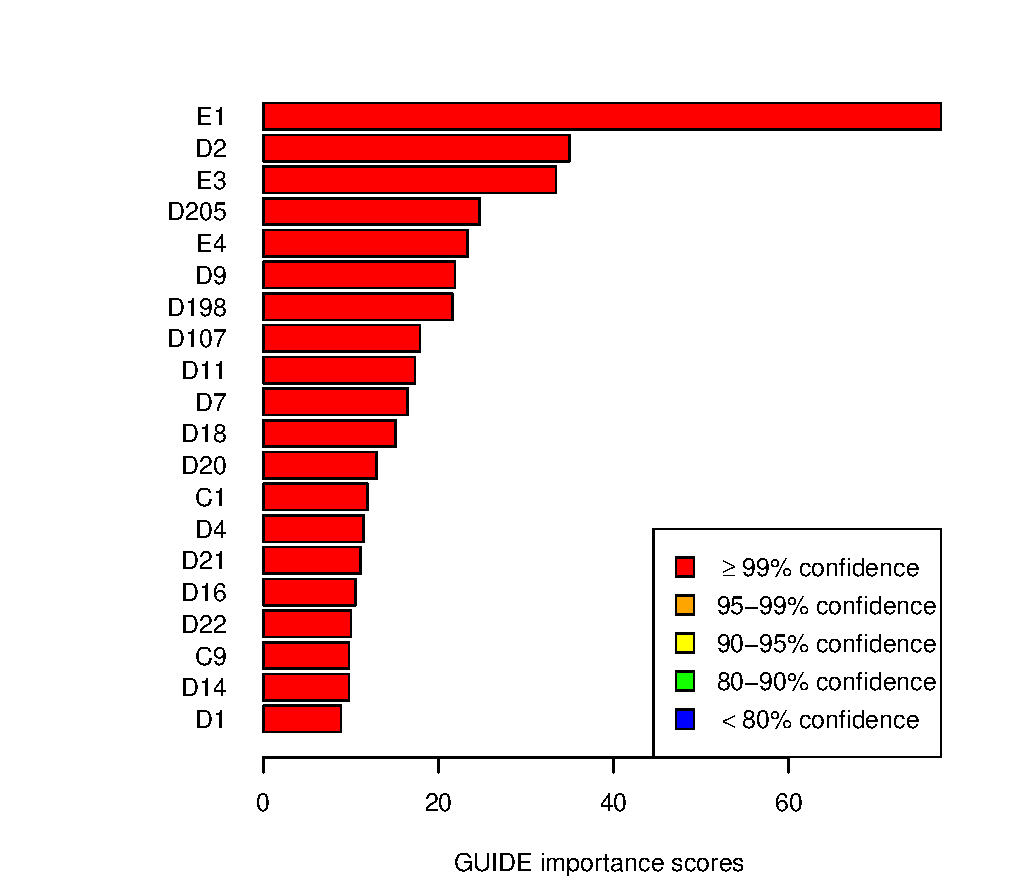
\includegraphics[scale=0.32]{A2_imp.eps} \label{1}
    }
    \subfigure[年龄与生活、饮食习惯的决策树可视化]{
    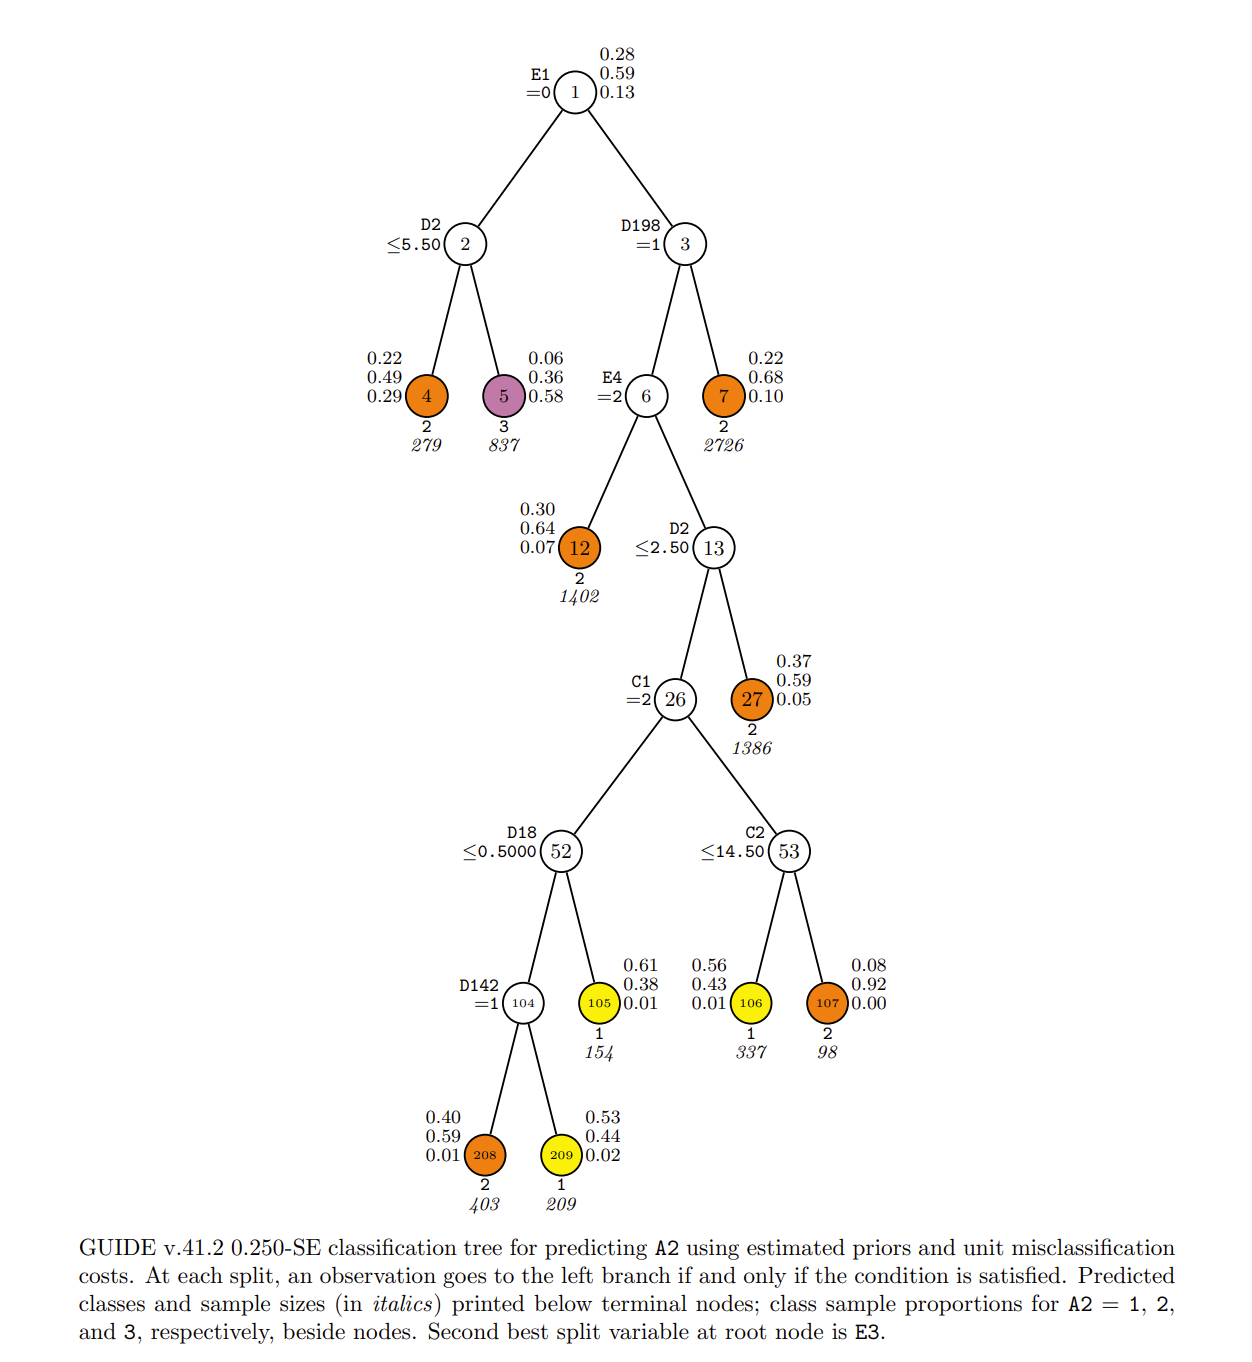
\includegraphics[scale=0.32]{A2_tree.png} \label{2} 
    }
    \quad
    \caption{A2年龄与生活、饮食习惯决策树结果}
\end{figure}

可以看到E1,D2,E3,D205,E4因素对分类结果影响较大,即不同年龄的人在工作属于的活动、一周在家吃早餐的次数、是否参加体育锻炼、是否吃其它饮料、是否参加体育锻炼在这些方面差异较大。通过决策树模型我们也可以发现:18-45岁的青年人群主要从事中重度的工作,喝果汁,体育锻炼强度大,一周在家吃早餐的天数少($\leq$2),其中不饮酒的人更愿意在单位食堂吃晚餐且不爱吃干豆。46-69的中年人群体分支较多:中年人中的离退休人群较老年人不爱在家中吃早饭;仍在工作的中年人较不爱喝果汁,体育锻炼强度小,较青年人爱在家吃早饭,也更爱吃干豆。老年人群体一周在家吃早餐的时间在6天以上。
\subsubsection{A3性别与生活、饮食习惯}
我们得到GUIDE决策树算法中自变量与因变量性别之间相关性的评分,以下是分类置信度>99\%的前20名变量与决策树可视化。
\begin{figure}[htbp]
    \centering
    \subfigure[性别vs生活、饮食习惯变量的重要性排名]{
    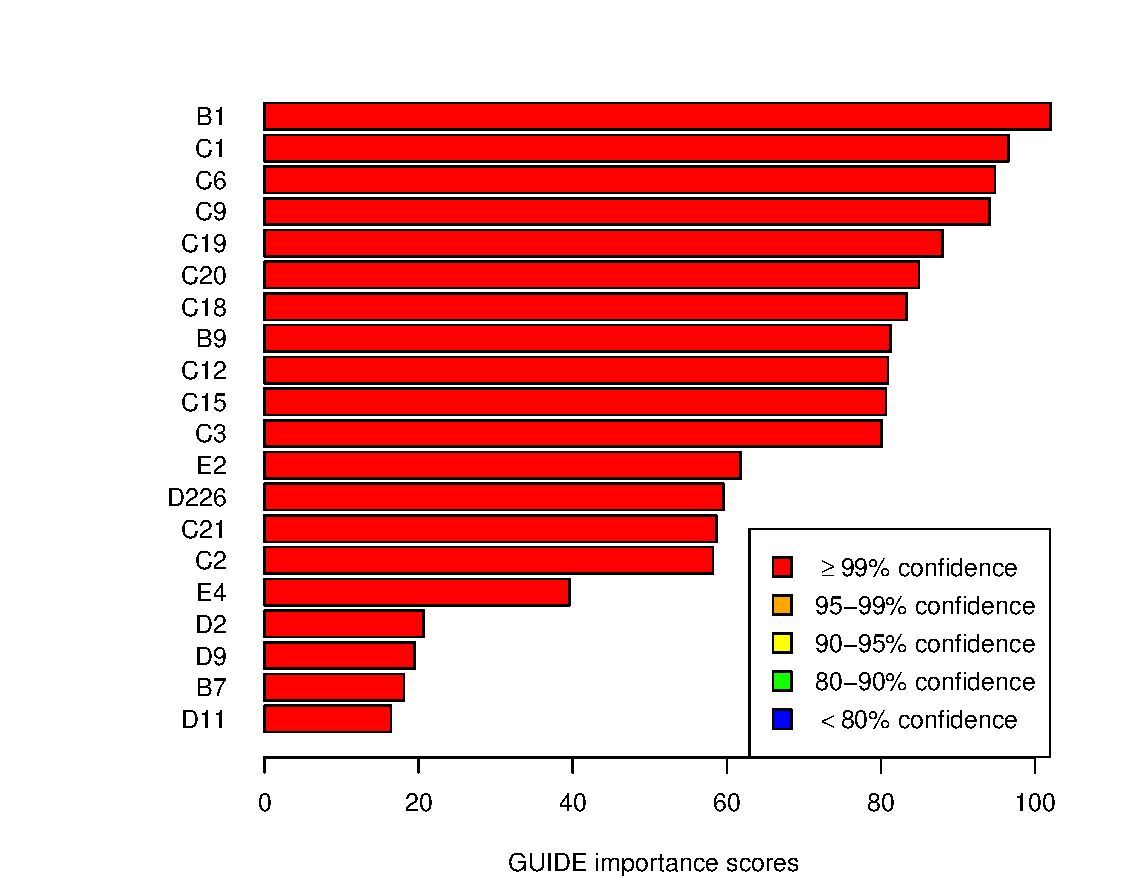
\includegraphics[scale=0.3]{A3_imp.eps} \label{1}
    }
    \subfigure[性别与生活、饮食习惯的决策树可视化]{
    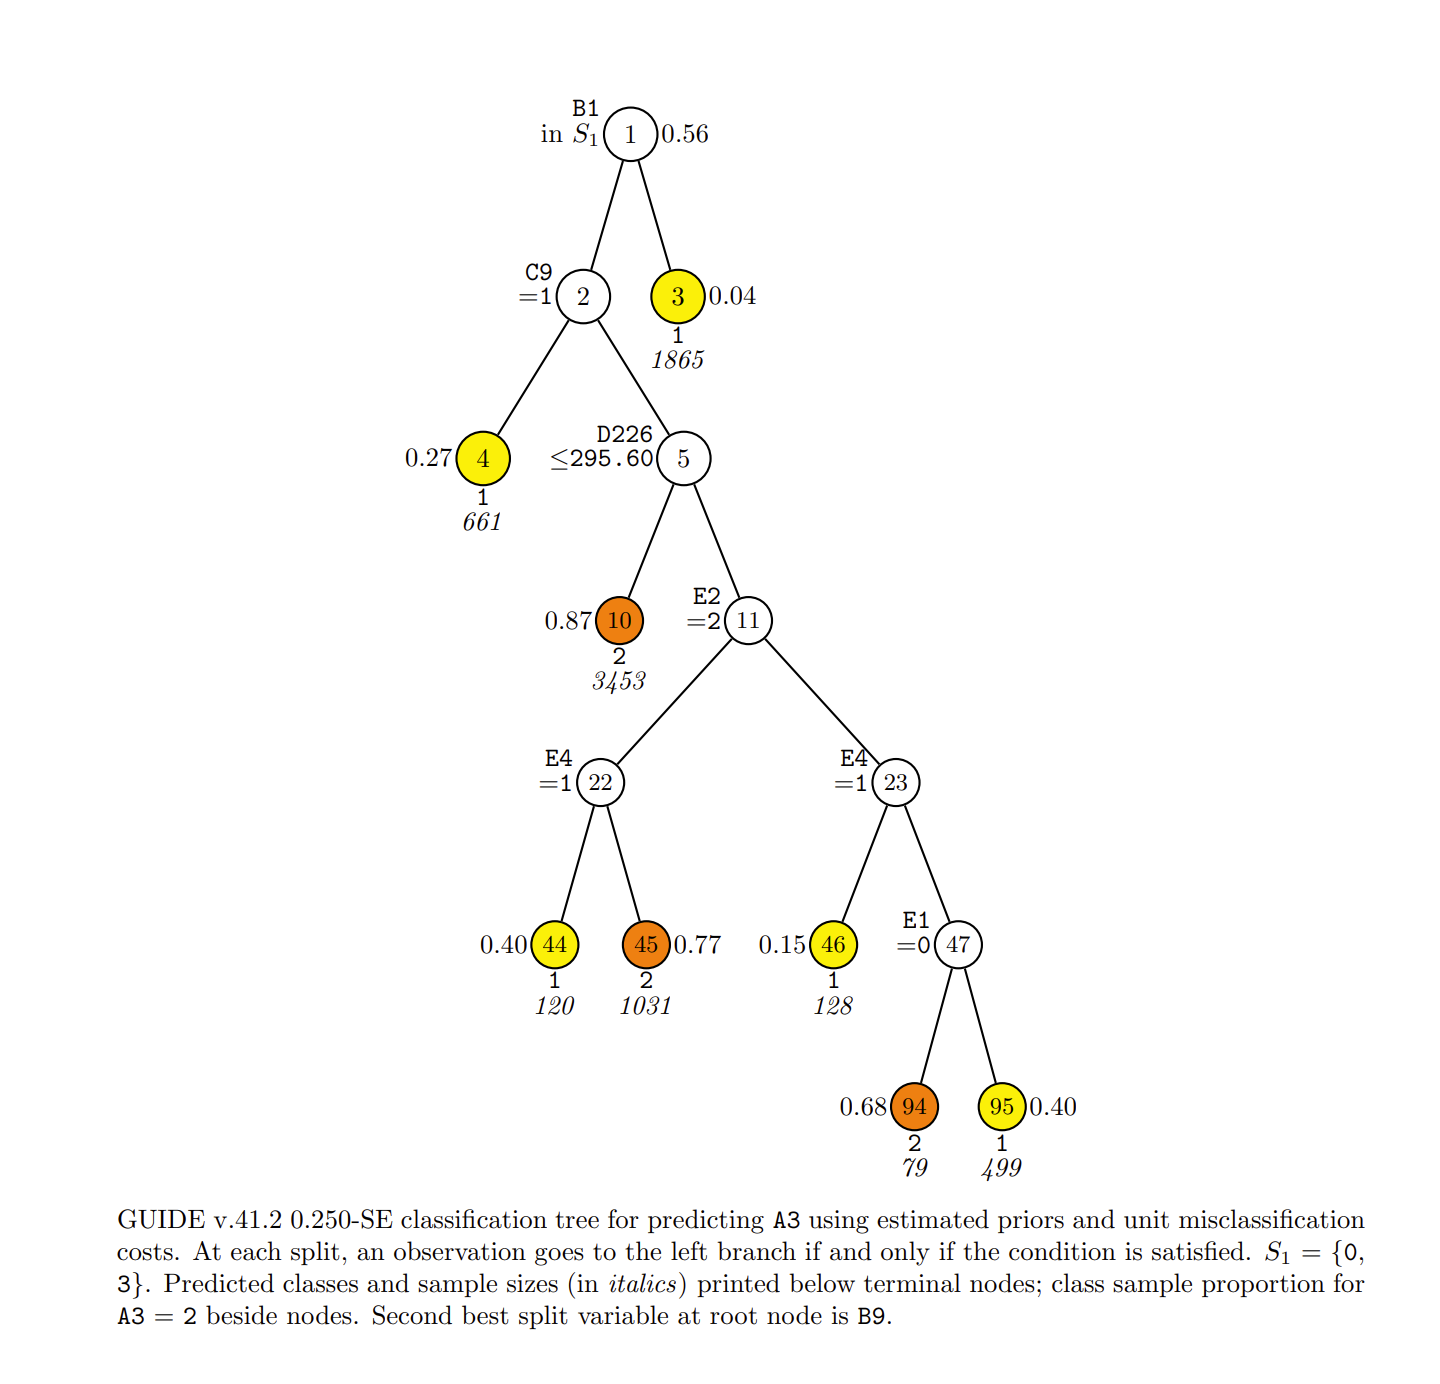
\includegraphics[scale=0.3]{A3_tree.png} \label{2} 
    }
    \quad
    \caption{A3性别与生活、饮食习惯决策树结果}
\end{figure}

可以看到因素B1是否吸烟、C1是否饮酒、C6是否饮用低度白酒、C9是否饮用啤酒、C19 度数加权平均每次饮酒量、C20每周饮用酒精量对分类结果影响比较大。通过决策树模型我们可以发现,男性在生活习惯上,较女性更会养成吸烟、饮酒的习惯。有意思的是,男性谷薯类食物的摄入量较高,即男性在主食上食用量较大。
\subsubsection{A6文化程度与生活、饮食习惯}
我们得到GUIDE决策树算法中自变量与因变量文化程度之间相关性的评分,以下是分类置信度>99\%的前20名变量与决策树可视化。
\begin{figure}[htbp]
    \centering
    \subfigure[文化程度vs生活、饮食习惯变量的重要性排名]{
    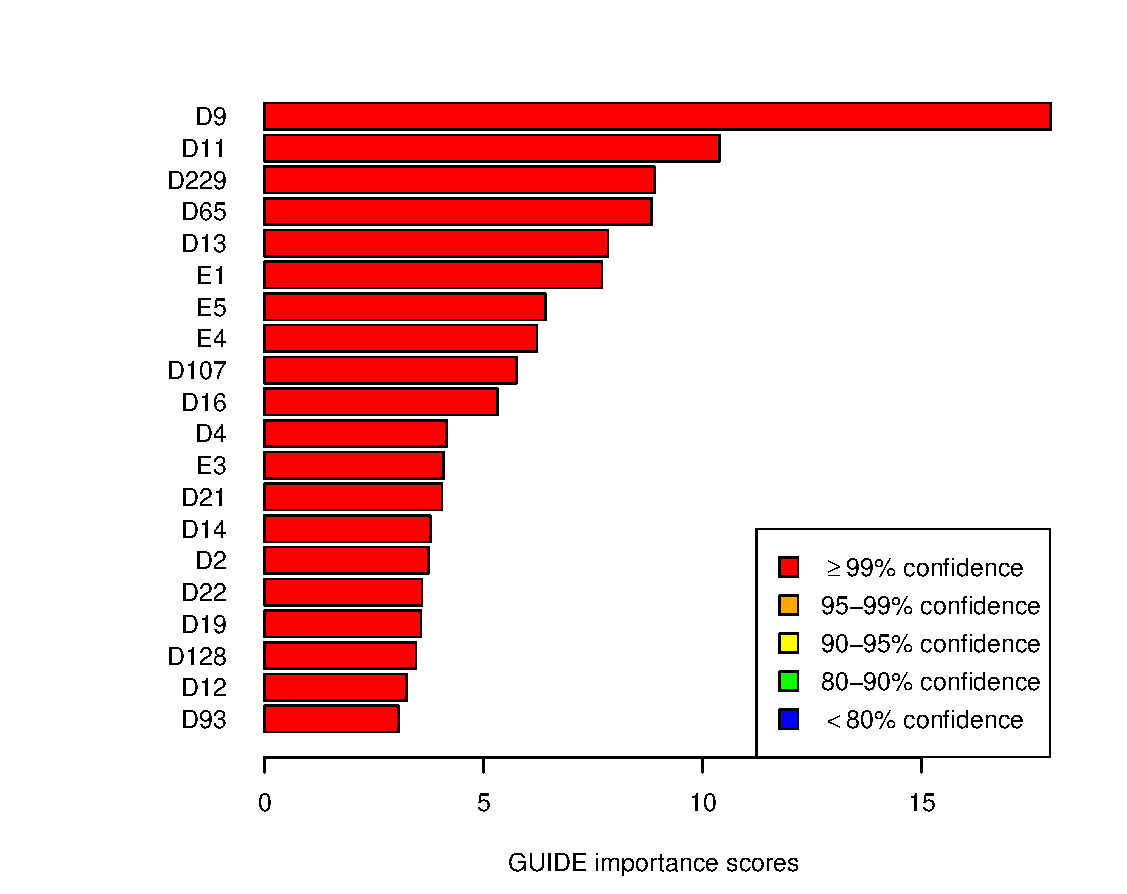
\includegraphics[scale=0.3]{A6_imp.eps} \label{1}
    }
    \subfigure[文化程度与生活、饮食习惯的决策树可视化]{
    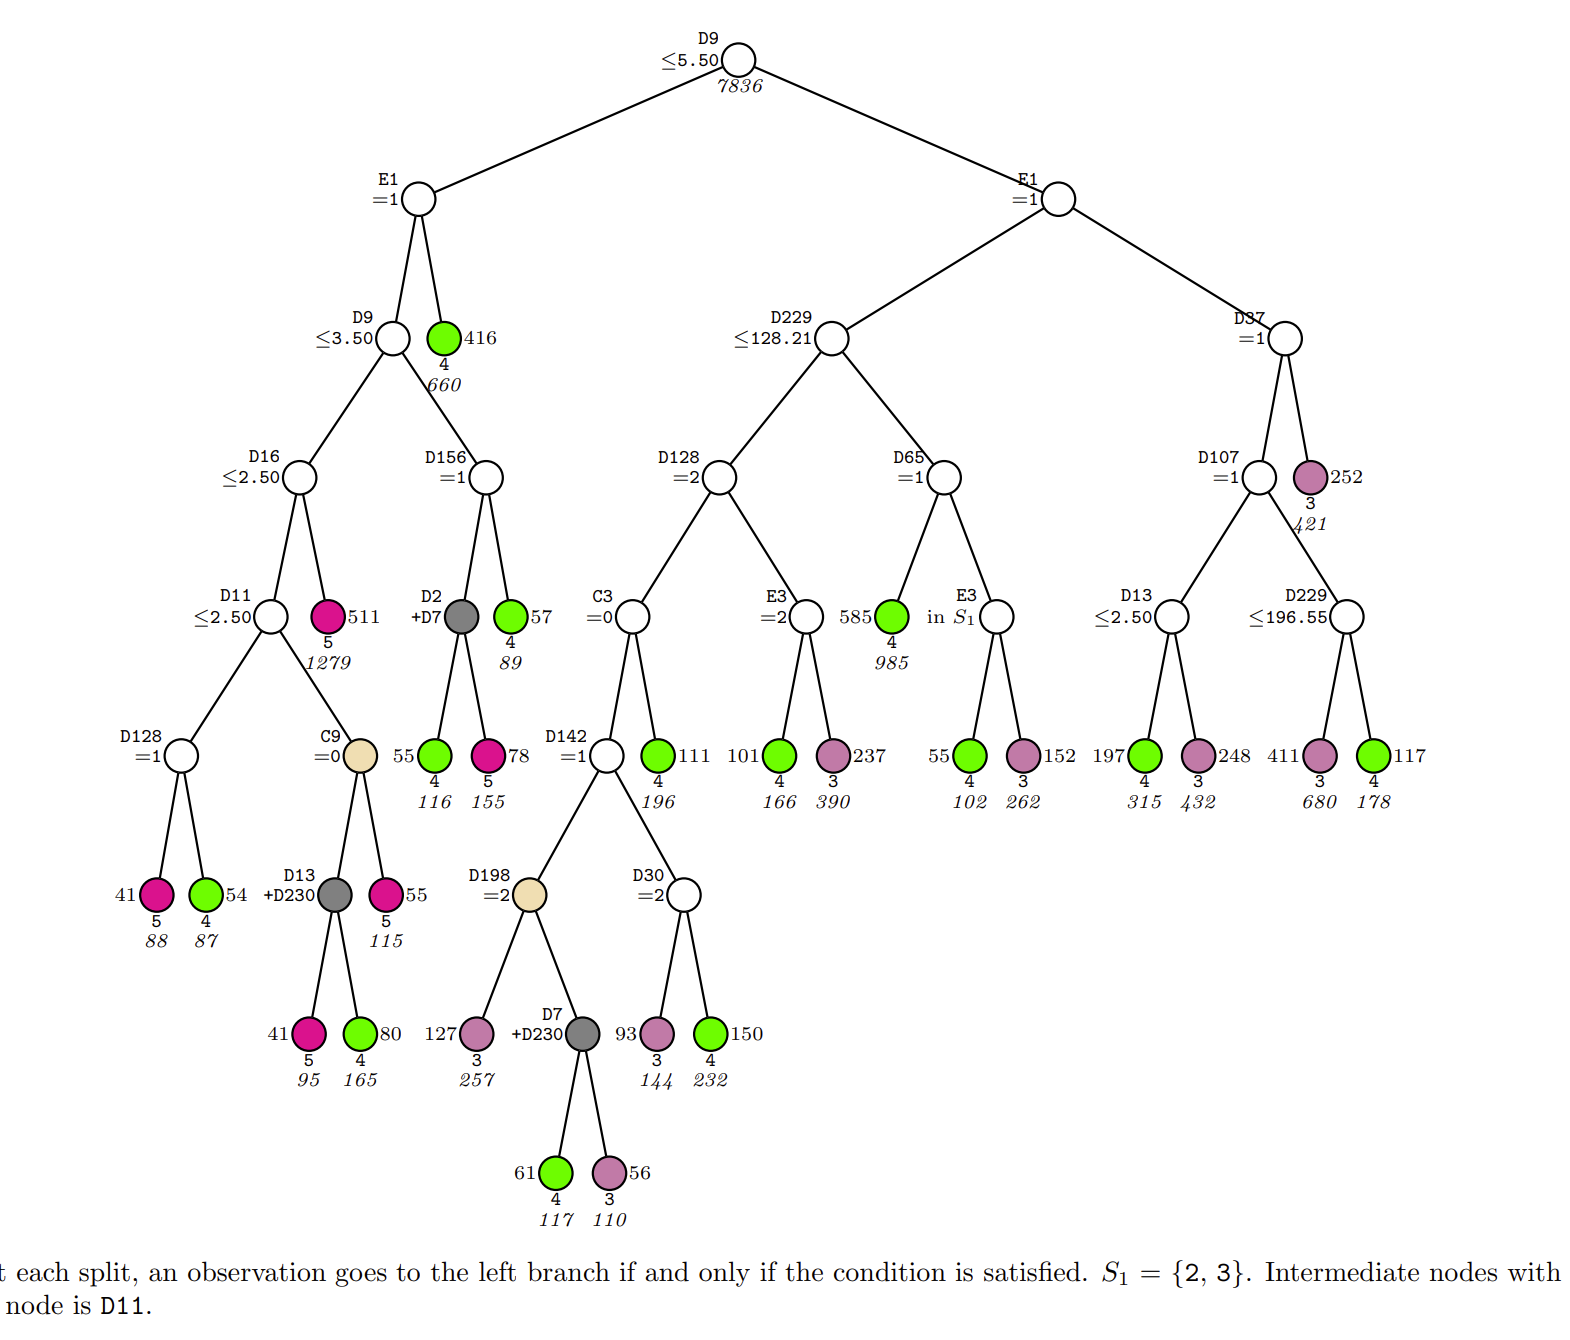
\includegraphics[scale=0.257]{A6_tree.png} \label{2} 
    }
    \quad
    \caption{A6文化程度与生活、饮食习惯}
\end{figure}

可以看到D9在家吃中餐、D11在单位食堂吃中餐、D229奶类大豆坚果制品、D65是否吃牛羊肉、D13工作日在家吃中餐人数、E1工作主要属于何种强度活动、E5平均每天体育锻炼时间对分类结果影响比较大。侧面说明文化程度越高的居民,午餐更倾向规律,并且工作强度倾向较低,日常锻炼时间倾向较少。
\subsubsection{A7婚姻状况与生活、饮食习惯}
我们得到GUIDE决策树算法中自变量与因变量婚姻状况之间相关性的评分,以下是分类置信度>99\%的前20名变量与决策树可视化。
\begin{figure}[htbp]
    \centering
    \subfigure[婚姻状况vs生活、饮食习惯的重要性排名]{
    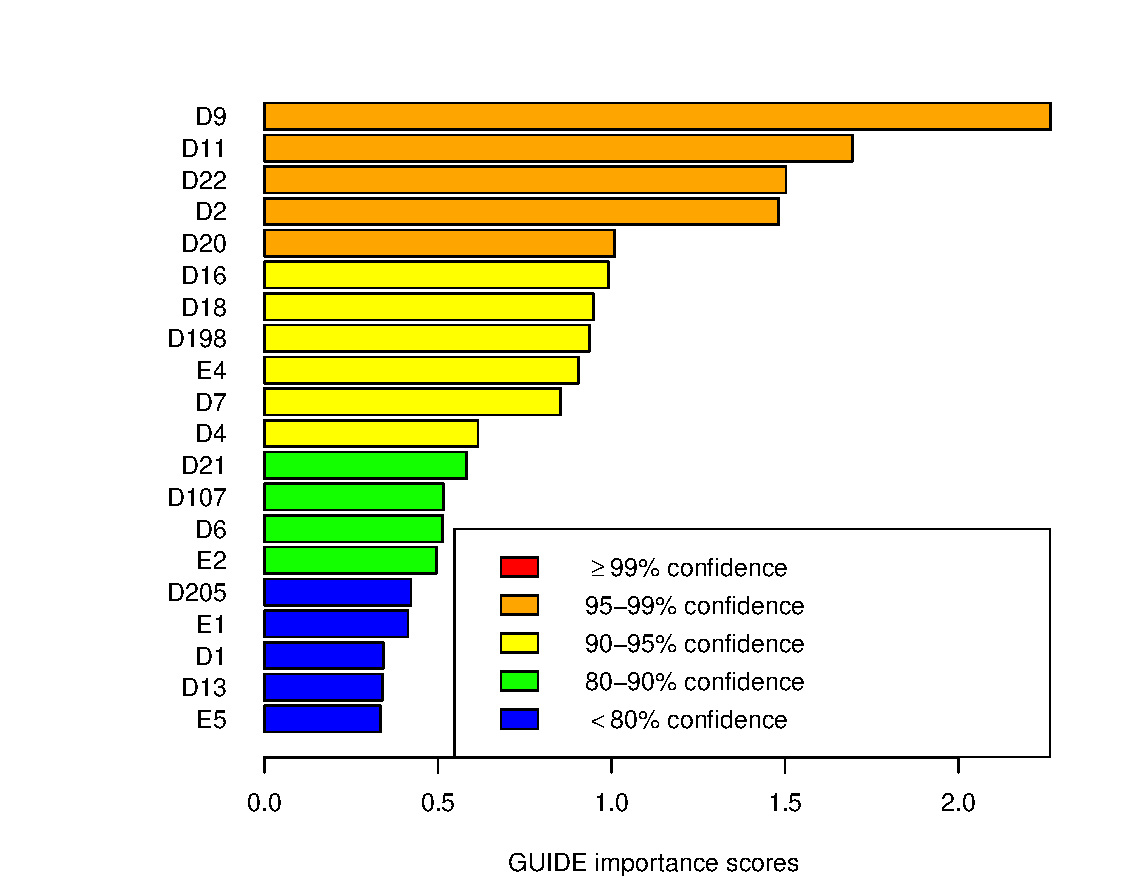
\includegraphics[scale=0.3]{A7_imp.eps} \label{1}
    }
    \subfigure[婚姻状况与生活、饮食习惯的决策树可视化]{
    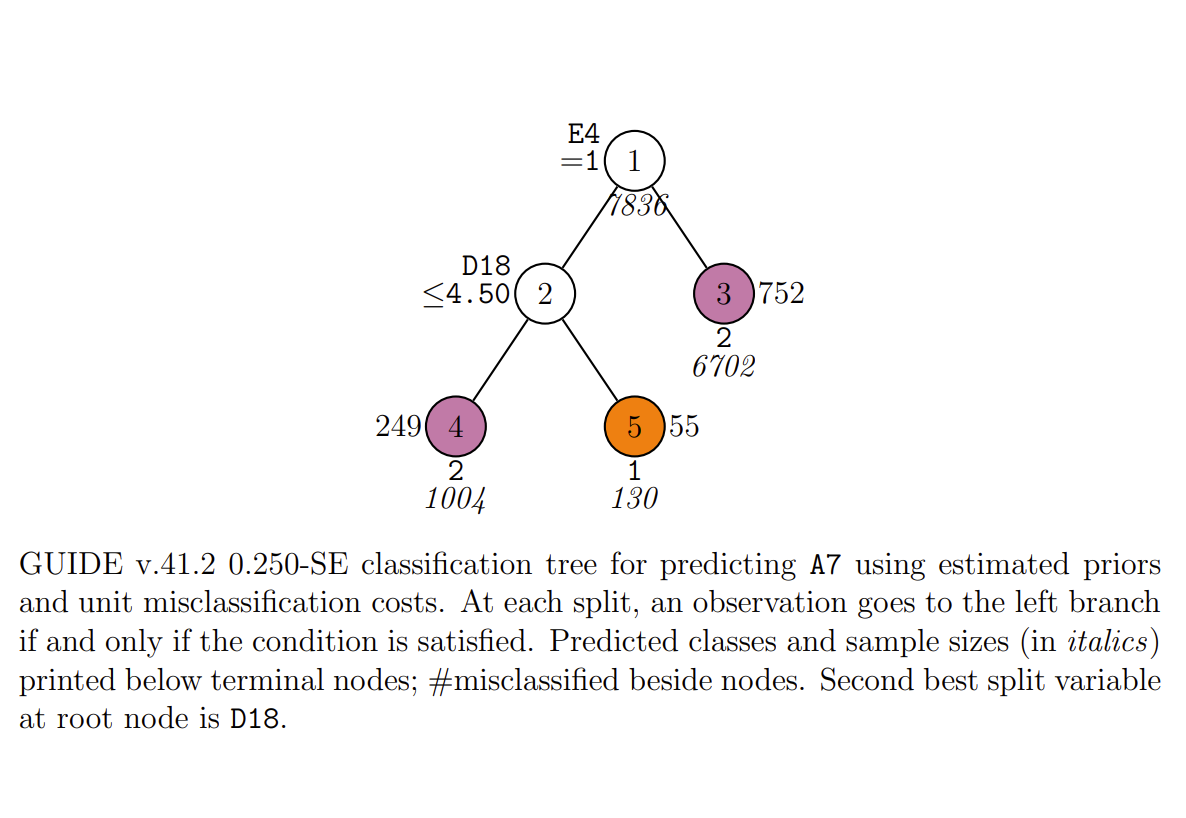
\includegraphics[scale=0.43]{A7_tree.png} \label{2} 
    }
    \quad
    \caption{A6文化程度与生活、饮食习惯}
\end{figure}

可以看到未婚人群中参与高强度的体育体育锻炼的人明显更多,且更倾向于在单位食堂吃晚餐;已婚人群更倾向于在家中吃晚餐,且更倾向于做中低强度的运动。
\subsubsection{A8职业与生活、饮食习惯}
我们得到GUIDE决策树算法中自变量与因变量职业之间相关性的评分,以下是分类置信度>99\%的前20名变量与决策树可视化。
\begin{figure}[htbp]
    \centering
    \subfigure[职业vs生活、饮食习惯变量的重要性排名]{
    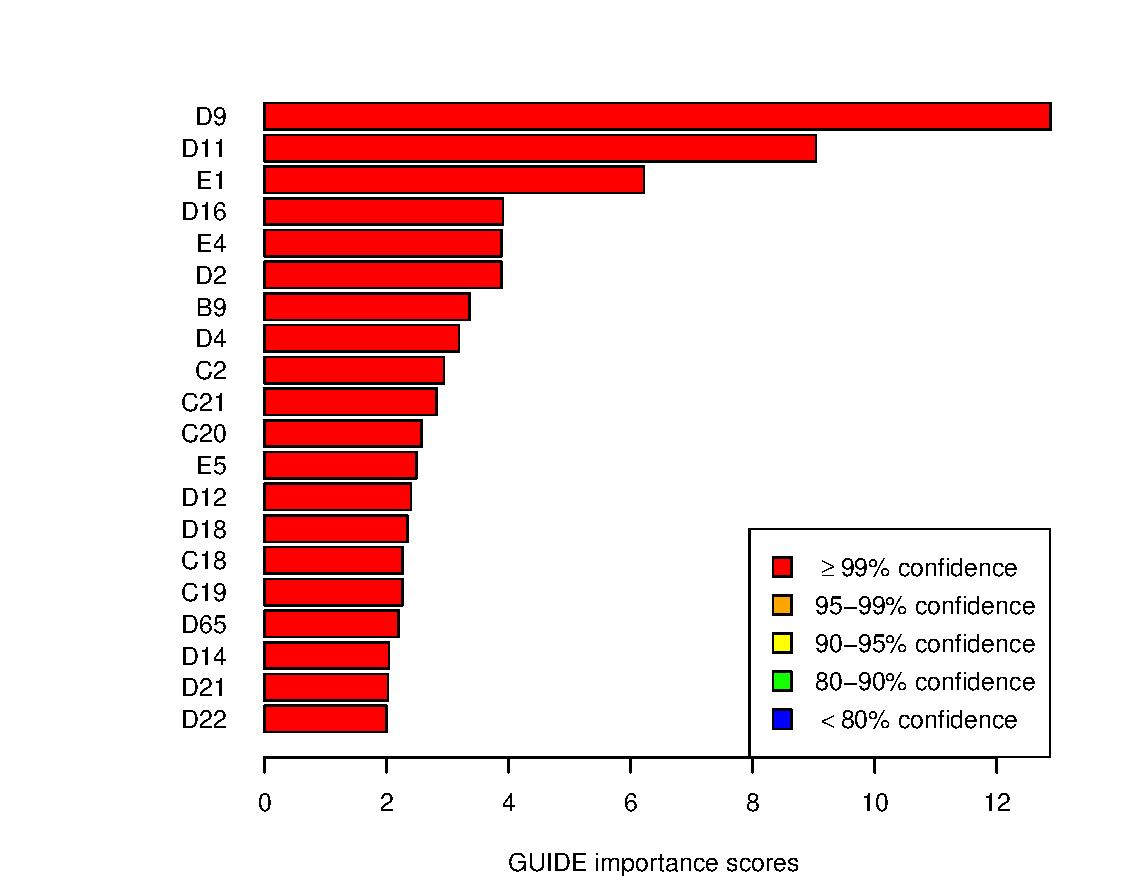
\includegraphics[scale=0.3]{A8_imp.eps} \label{1}
    }
    \subfigure[职业与生活、饮食习惯的决策树可视化]{
    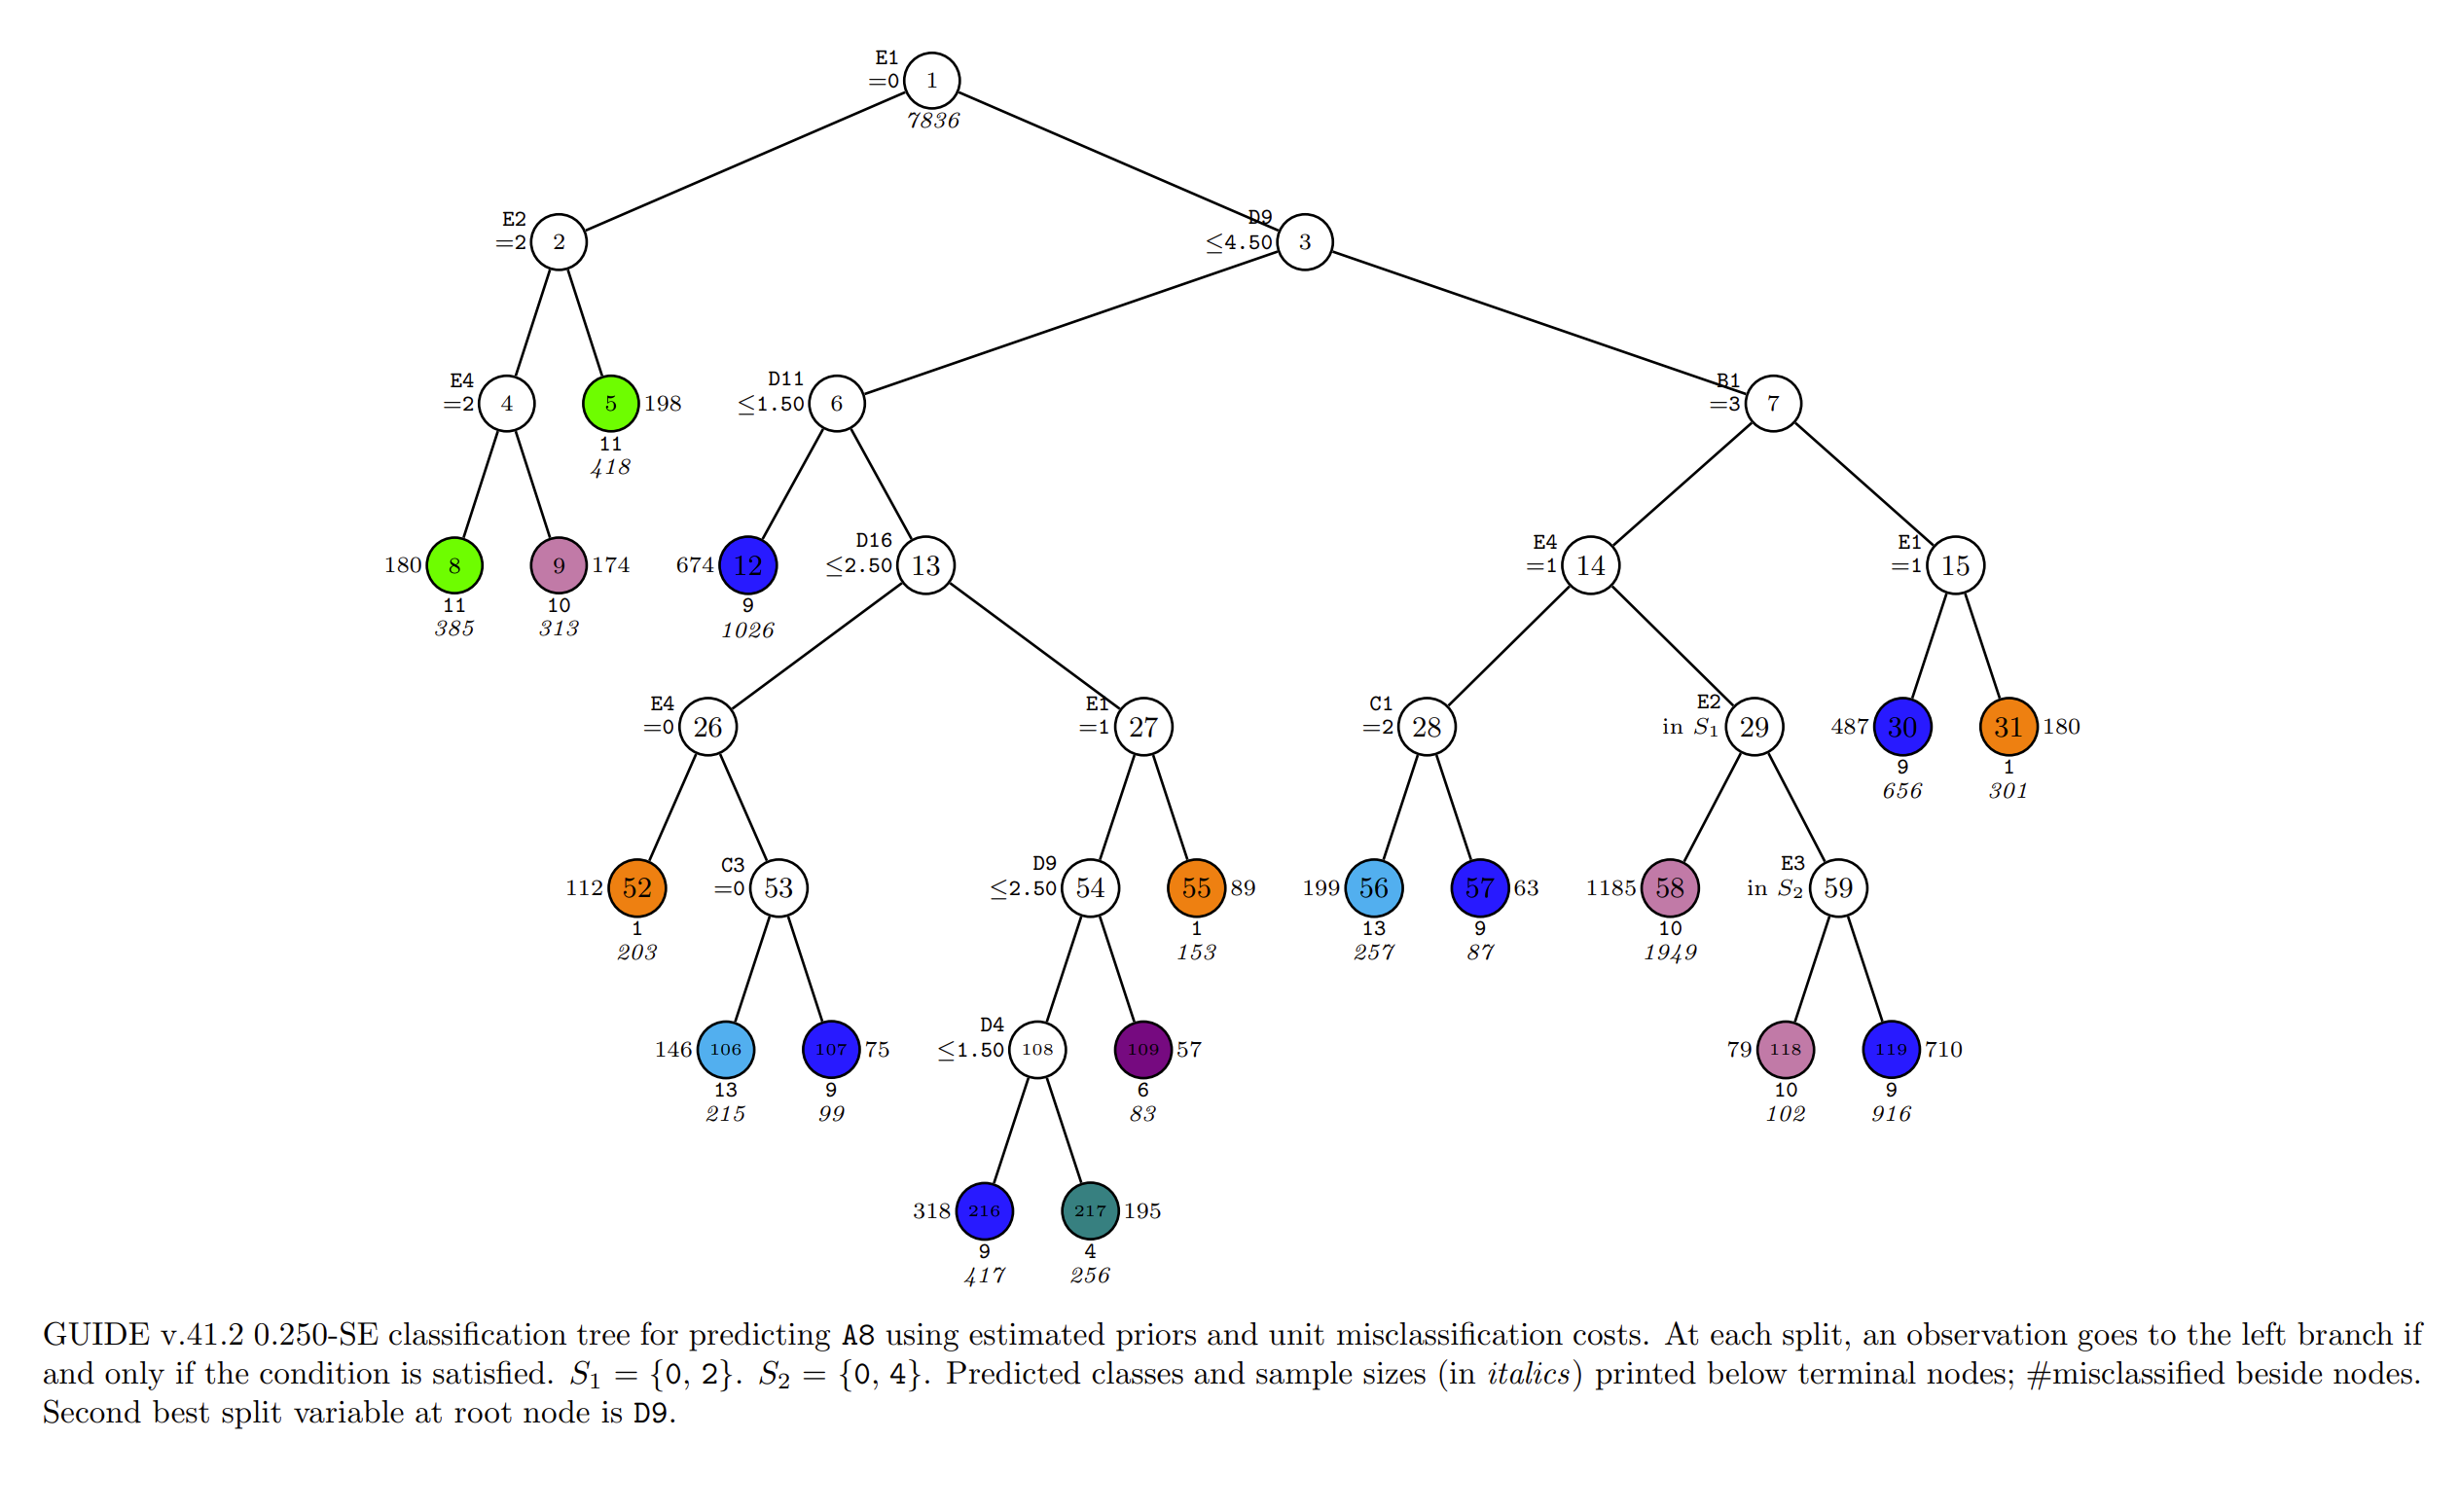
\includegraphics[scale=0.25]{A8_tree.png} \label{2} 
    }
    \quad
    \caption{A8职业与生活、饮食习惯}
\end{figure}

可以看到D9在家吃中餐、D11在单位食堂吃中餐、E1工作主要属于何种强度活动、D16在家吃晚饭、E4体育锻炼的强度、D2在家吃早饭对分类结果影响比较大。从中说明,不同的职业,中餐晚餐食用地点差别较大,工作强度差别较大,日常体育锻炼的强度差异较大。学生的体育锻炼强度大,且在家中的休闲劳动强度也较大;工人几乎不参加体育锻炼(E4=0),一日三餐很少在家中吃,有趣的是在家中吃饭的工人几乎都有烟史;家庭妇女大部分的活动大部分都是中度家务,且有趣的是家庭妇女要么一周运动>5天,要么不参加锻炼,可能是由于部分居民认为家务也是锻炼的一部分。行政干部大都选择早上和中午在食堂就餐,晚上回家吃晚饭;商业服务人员有饮酒史的多,他们的三餐就餐地点比较多样化,且大部分都有锻炼的习惯。

%============================================================================================================
{\centering\section{问题三的建模与求解}}
\subsection{模型建立}
根据世界卫生组织发布的指南,从受试者体检指标中得到受试者四种慢性病的情况。

\textbf{慢病1.}高血压:收缩压$\geq$140mmHg并且舒张压$\geq$90mmHg

\textbf{慢病2.}糖尿病:空腹血糖$\geq$ 7.0 mmol/L

\textbf{慢病3.}高血脂:总胆固醇 $\geq$ 6.2mmol/L 或者 高密度脂蛋白 < 1.0 mmol/L 或者 低密度脂蛋白 $\geq$ 24.1 mmol/L 或者 总甘油三酯 $\geq$ 2.3mmol/L

\textbf{慢病4.}高尿酸血症:血尿酸$\geq$ 420μmol/L

将得某慢性病的居民在对应列记作1,未得病则记作0。
建立logistic二分类回归模型,探究慢性病和与吸烟、饮酒、饮食习惯、生活习惯、工作性质、运动等因素的关系以及相关程度。
\begin{equation}
    \text{logistic回归:}\ln (\frac{P(Y=1)}{1-P(Y=1)}) = a_0 + \sum_{i=1}^{n}a_iX_i
\end{equation}
利用最小二乘法计算系数大小,从而得到$X_i$与$Y$的相关性,进一步可得相关性显著程度。

\subsection{模型求解与结论}

\subsubsection{高血压(占比5.2\%)}

首先考虑所有可能有关变量,得到logistic回归数据(详见附录3.1)

观察显著性p值可知:亲人是否有得过高血压、腰围、体重、是否饮酒、饮酒年数、酒精度数加权饮用频率、不吃晚餐会对高血压产生显著的正向影响关系,出生年份会对高血压产生显著的负向影响关系,其他因素并不会对高血压产生显著影响。
删去影响不显著的变量,再做一次logistic回归,得到:

\begin{figure}[H]
    \centering
    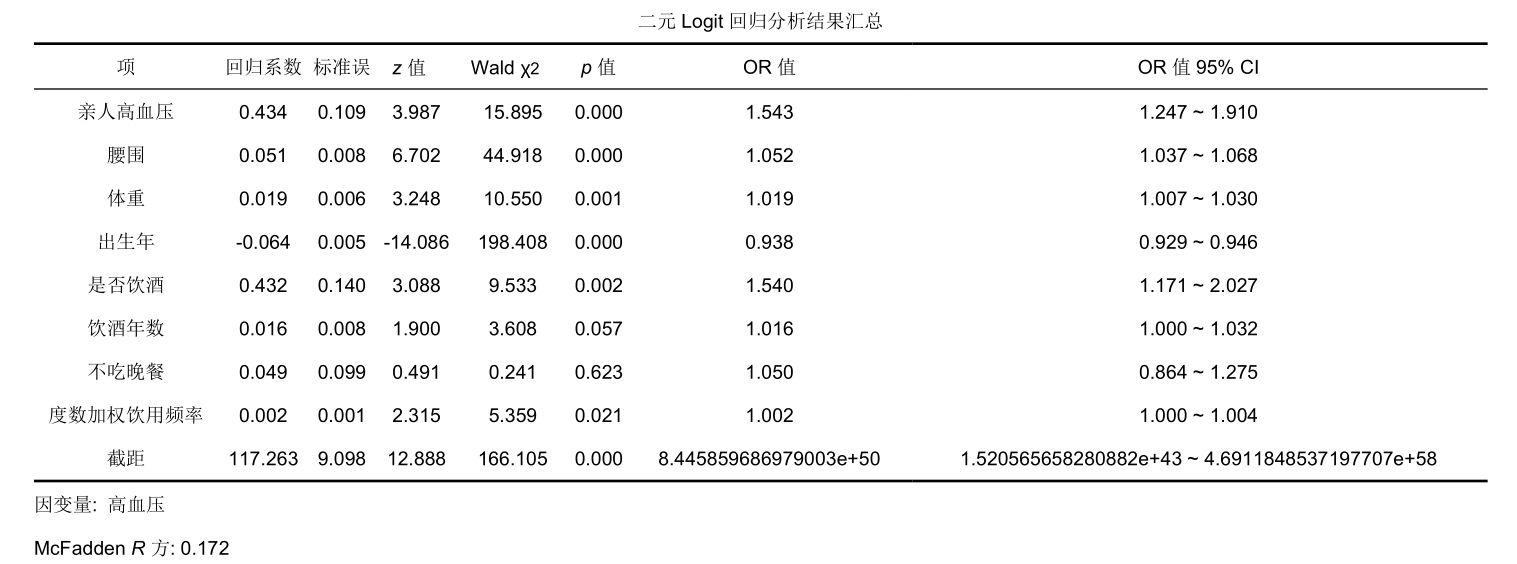
\includegraphics[scale=0.78]{logit2.png}
    \caption{高血压数据第二次logistic回归结果}
\end{figure}

通过二次logit回归数据总结得:

\begin{equation*}
    \begin{aligned}
        \ln(\frac{P(\text{得高血压})}{1-P(\text{得高血压})})
        =&117.263 + 0.434*\text{亲人是否得过高血压} + 0.051*\text{腰围}\\
        & + 0.019*\text{体重}-0.064*\text{出生年} + 0.432*\text{是否饮酒} \\
        &+ 0.016*\text{饮酒年数} + 0.049*\text{不吃晚餐} + 0.002*\text{酒精度数加权饮酒频率}\\
    \end{aligned}
\end{equation*}
%$$\ln(\frac{P(\text{得高血压})}{1-P(\text{得高血压})})=117.263 + 0.434*\text{亲人是否得过高血压} + 0.051*\text{腰围}\\+ 0.019*\text{体重}-0.064*\text{出生年} + 0.432*\text{是否饮酒} + 0.016*\text{饮酒年数} + 0.049*\text{不吃晚餐} + 0.002*\text{酒精度数加权饮酒频率}$$

\subsubsection{糖尿病(占比2.9\%)}

首先考虑所有可能有关变量,得到logistic回归数据(详见附录3.2)。

观察显著性p值可知:腰围、烹调油盐、腌制品、亲人是否得过糖尿病会对糖尿病产生显著的正向影响关系,出生年、臀围、谷薯类食物会对糖尿病产生显著的负向影响关系,其他因素并不会对糖尿病产生显著影响。此外,由于臀围与实际情况过于不符,故删去。
删去影响不显著的变量,再做一次logistic回归,得到:

\begin{figure}[H]
    \centering
    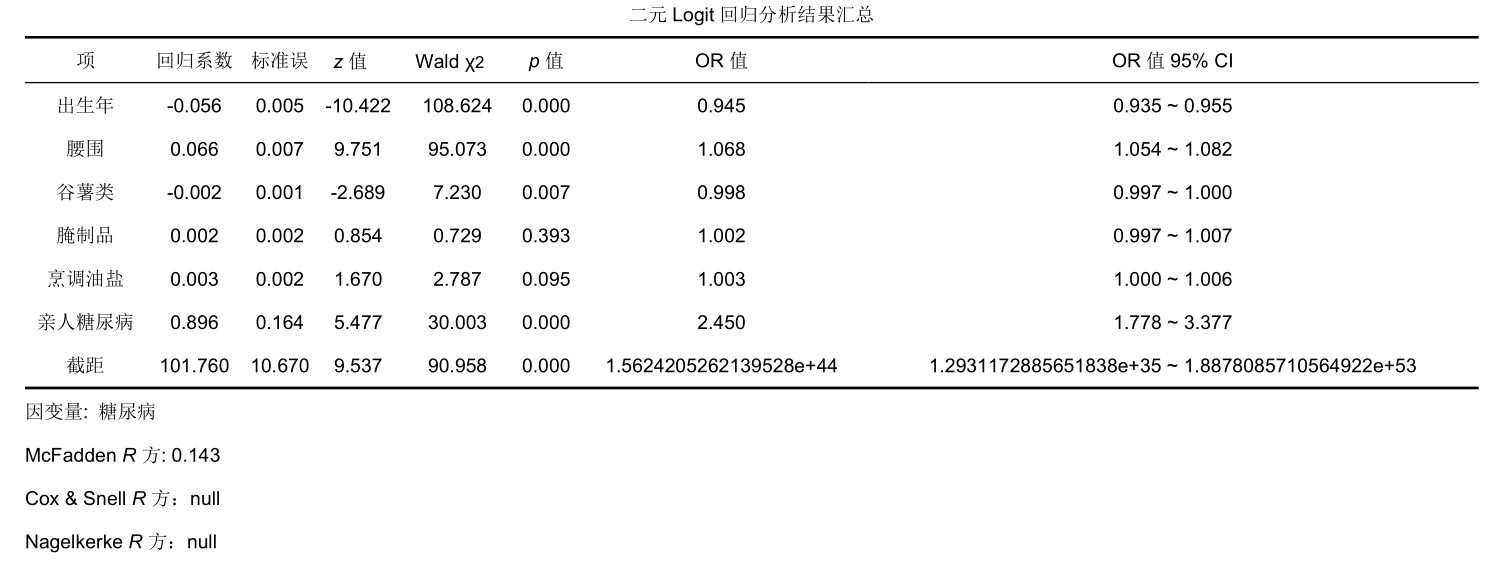
\includegraphics[scale=0.78]{logit4.png}
    \caption{糖尿病数据第二次logistic回归结果}
\end{figure}

通过二次logit回归数据总结得:
\begin{equation*}
    \begin{aligned}
        \ln(\frac{P(\text{得糖尿病})}{1-P(\text{得糖尿病})})
        =&101.760-0.056*\text{出生年} + 0.066*\text{腰围}-0.002*\text{谷薯类} \\
        &+ 0.002*\text{腌制品} + 0.003*\text{烹调油盐} + 0.896*\text{亲人糖尿病}\\
    \end{aligned}
\end{equation*}

\subsubsection{高血脂(占比32.9\%)}
由上同理,我们可知:腰围, 体重, 是否饮酒会对高血脂产生显著的正向影响关系,以及出生年, 性别, 身高, 工作主要属于以下何种活动会对高血脂产生显著的负向影响关系。其他因素印象较小。二次处理,得到:

\begin{equation*}
    \begin{aligned}
        \ln(\frac{P(\text{得高血脂})}{1-P(\text{得高血脂})})
        =&32.191-0.017*\text{出生年} + 0.056*\text{腰围}-0.866*\text{性别} + 0.012*\text{体重}\\&-0.021*\text{身高}-0.139*\text{工作主要属于以下何种活动} + 0.105*\text{是否饮酒}
    \end{aligned}
\end{equation*}

\subsubsection{高尿酸血症(占比8.4\%)}

出生年, 腰围会对高尿酸血症产生显著的正向影响关系,以及性别, 您做休闲、家务活动的强度, 烹调油盐会对高尿酸血症产生显著的负向影响关系。

\begin{equation*}
    \begin{aligned}
        \ln(\frac{P(\text{得高尿酸血症})}{1-P(\text{得高尿酸血症})})
        =&-26.727 + 0.011*\text{出生年} + 0.060*\text{腰围}-1.688*\text{性别}\\
        &-0.307*\text{您做休闲、家务活动的强度}-0.006*\text{烹调油盐}
    \end{aligned}
\end{equation*}

%============================================================================================================
{\centering\section{问题四的建模与求解}}
\subsection{居民分类}
根据问题一与问题三的结论,我们可以将人群大致分为以下几类:
\subsubsection{慢性病患者}
患有一种或多种下列慢性疾病:

\textbf{1.}高血压:收缩压$\geq$140mmHg并且舒张压$\geq$90mmHg

\textbf{2.}糖尿病:空腹血糖$\geq$ 7.0 mmol/L

\textbf{3.}高血脂:总胆固醇 $\geq$ 6.2mmol/L 或者 高密度脂蛋白 < 1.0 mmol/L 或者 低密度脂蛋白 $\geq$ 24.1 mmol/L 或者 总甘油三酯 $\geq$ 2.3mmol/L

\textbf{4.}高尿酸血症:血尿酸$\geq$ 420μmol/L

\subsubsection{潜在慢性病患者}
非慢性病患者,但满足一种或多种下列条件:

\textbf{1.}P(得高血压)>5.2\%为潜在高血压患者

\textbf{2.}P(得糖尿病)>2.9\%为潜在糖尿病(高血糖)患者

\textbf{3.}P(得高血脂)>32.9\%为潜在高血脂患者

\textbf{4.}P(高尿酸血症)>8.4\%为潜在高尿酸血症患者

\subsubsection{习惯不合理的健康居民}
非上述两类人群,但满足一种或多种下列条件:

\textbf{1.}吸烟

\textbf{2.}度数加权饮酒频率>34.5

\textbf{3.}问题一中膳食结构违背标准

\textbf{4.}运动量低于标准

\textbf{5.}BMI不在标准区间

\subsubsection{习惯合理的健康居民}
非上述三类人群

\subsection{合理建议}
\subsubsection{患者与潜在患者}

\textbf{1.}高血压:饮食要规律(吃晚饭),控制酒精和脂肪摄入、多加运动(控制体重和腰围)。

\textbf{2.}糖尿病:少吃油盐以及腌制品,多加锻炼,多吃粗粮。

\textbf{3.}高血脂:多加锻炼,日常提高运动量(从事高强度工作,控制体重),戒酒。

\textbf{4.}高尿酸血症:少吃烹调油盐,日常需要多加活动。

\subsubsection{健康居民}
\textbf{1.}戒烟,少饮酒。

\textbf{2.}多加运动(每周运动量达标),控制BMI(标准区间)。

\textbf{3.}保持合理的膳食结构(八条准则),多吃新鲜蔬果、奶制品,少吃油盐、腌制品。

\textbf{4.}足量饮水,保持健康规律的生活习惯和饮食习惯。

%============================================================================================================
{\centering\section{模型的评价与改进}}

\subsection{二元logistic回归模型}
\subsubsection*{(1)模型的优点}
1.模型简单,速度快,适合二分类问题;

2.简单易于理解,直接看到各个特征的权重;

3.能容易地更新模型吸收新的数据;
\subsubsection*{(2)模型的缺点}
1.学习能力较弱,对数据和场景的适应能力有局限性;

2.容易忽视变量之间的相关性,在强相关的因素下,一些弱相关的因素会被淹没;

3.不患病和患病居民数量级差距太大,造成样本特征被淹没。
\subsubsection*{(3)模型的改进}
1.用主成分分析进行数据降维,将几个大类用主成分分析归为部分抽象变量看待。

2.给慢性病按照病情严重程度分3档或者5档,增加模型预测能力。

3.使用SMOTE(合成少数类过采样技术)分析少数样本并人工合成新样本添加入数据集,以缓解类别不平衡影响的模型输出

\subsection{GUIDE决策树模型}
\subsubsection*{(1)模型的优点}
1.可解释性强,可视化能力强,分类处理一目了然。

2.通过对不同的自变量进行数值型与类别型的分类,极大地保留了变量本身离散与连续的属性。

\subsubsection*{(2)模型的缺点}
1.决策树算法对变量之间可能存在的相关性无法阐明,可能会造成与因变量联系较强的
相关类型的变量只有一种脱颖而出,因此某些人群的较不明显的属性无法一并
体现。

2.自变量维度过高,决策树算法分类容易省略较多自变量与因变量的相
关信息。 
\subsubsection*{(3)模型的改进}
对多种自变量之间通过算法进行相关性分析,优化相似类型自变量,降维自变量模型


%============================================================================================================
{\centering\section{参考文献}}
\begingroup  % 去掉thebibliography环境自带的“参考文献”标题
\renewcommand{\section}[2]{}
\begin{thebibliography}{99}

\bibitem{1}
中国居民膳食指南.[中国居民膳食指南解读]中国居民平衡膳食宝塔(2022)修订和解析.[OL].(2023-8-17)[2023-8-17]. Retrieved from http://dg.cnsoc.org/article/04/RMAbPdrjQ6CGWTwmo62hQg.html

\bibitem{2}
Wikipedia.[Wikipedia]alcoholic drink[OL].(2023-8-17)[2023-8-17]. Retrieved from https://zh.wikipedia.org/wiki/alcoholic drink

\bibitem{4}The SPSSAU project (2023). SPSSAU. (Version 23.0) [Online Application Software]. Retrieved from https://www.spssau.com.

\bibitem{5}L. Breiman, J. Friedman, R. Olshen, and C. Stone. Classification and Regression Trees. Wadsworth, Belmont, CA, 1984.

\bibitem{6}T. Hastie, R. Tibshirani and J. Friedman. Elements of Statistical Learning, Springer, 2009.

\end{thebibliography}
\endgroup

%============================================================================================================
\newpage
{\centering\section*{附录}}
\appendix

\subsection*{1.问题一相关图像}
1.1问题1-1定量型膳食标准
\begin{figure}[htbp]
    \centering
    \subfigure[酒精摄入量散点图]{
    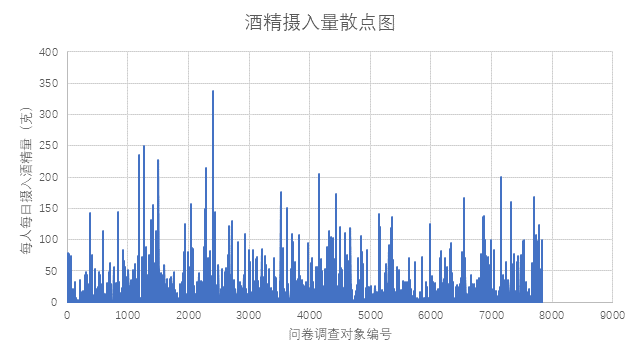
\includegraphics[scale=0.385]{1-1酒散点图.png} \label{1}
    }
    \subfigure[奶类摄入量散点图]{
    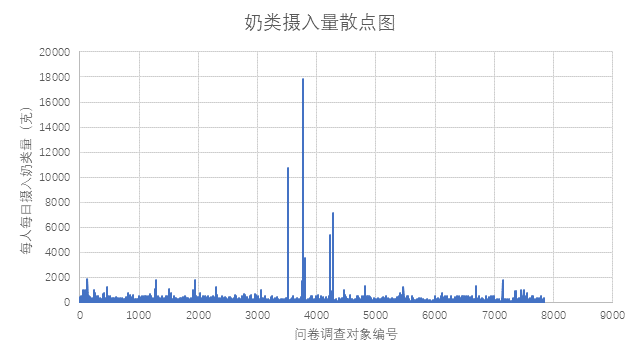
\includegraphics[scale=0.385]{1-1奶散点图.png} \label{2} 
    }
    \subfigure[油类摄入量散点图]{
    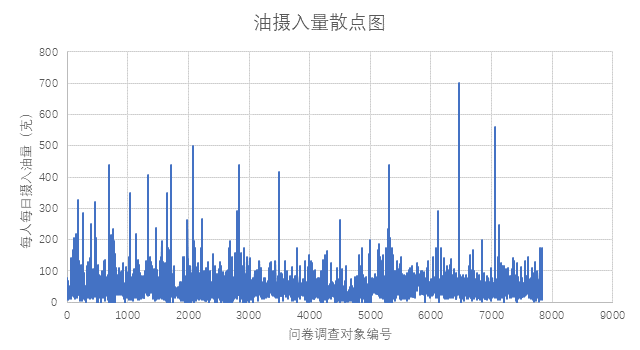
\includegraphics[scale=0.385]{1-1油散点图.png}\label{3}
    }
    \subfigure[新鲜蔬菜摄入量散点图]{
    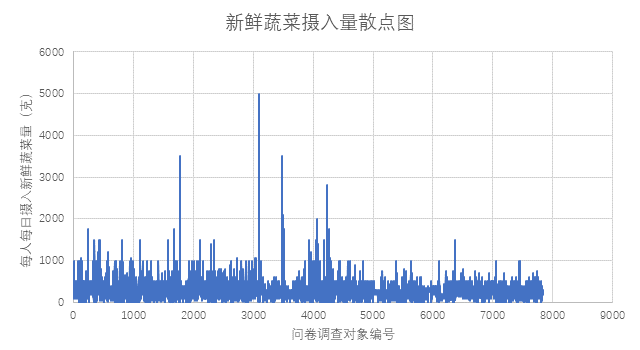
\includegraphics[scale=0.385]{1-1新鲜蔬菜散点图.png}\label{3}
    }
    \subfigure[新鲜水果摄入量散点图]{
    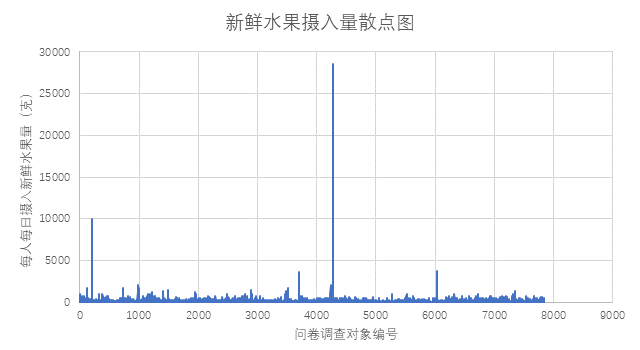
\includegraphics[scale=0.385]{1-1新鲜水果散点图.png}\label{3}
    }
    \subfigure[盐摄入量散点图]{
    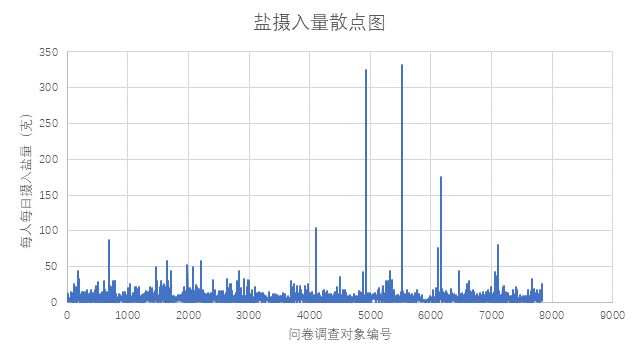
\includegraphics[scale=0.385]{1-1盐散点图.png}\label{3}
    }
    \subfigure[鱼禽蛋瘦肉摄入量散点图]{
    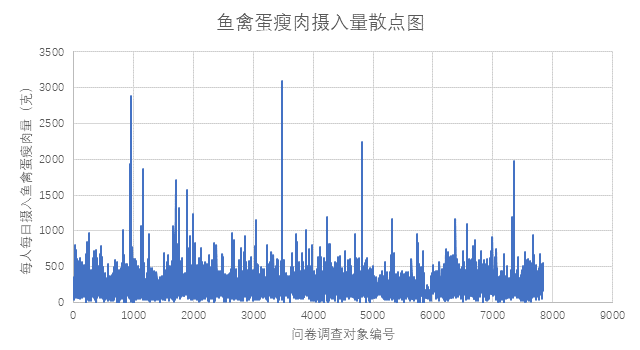
\includegraphics[scale=0.385]{1-1鱼禽蛋瘦肉散点图.png}\label{3}
    }
    \quad
    \caption{定量型膳食标准统计数据散点图}
\end{figure}
\newpage
1.2问题1-2非定量型膳食标准

\begin{figure}[htbp]
    \centering
    \subfigure[水产品摄入频率散点图]{
    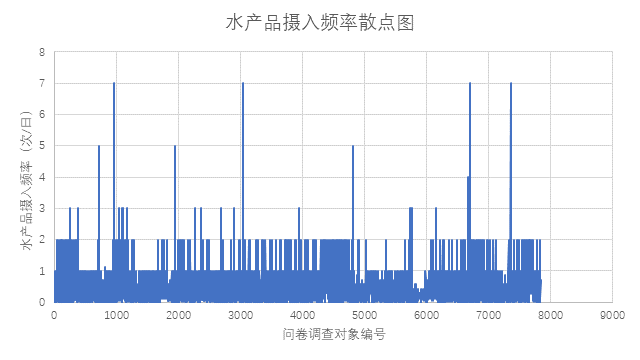
\includegraphics[scale=0.4]{1-2水产品散点图.png} \label{1}
    }
    \subfigure[蛋类摄入频率散点图]{
    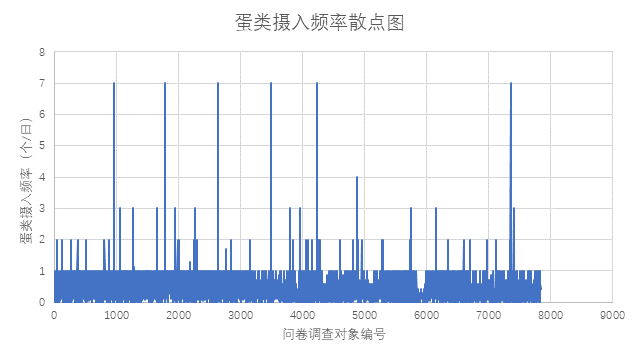
\includegraphics[scale=0.4]{1-2蛋类散点图.png} \label{2} 
    }
    \quad
    \caption{非定量型膳食标准统计数据散点图}
\end{figure}

\subsection*{2.问题二相关代码(R)}
绘制重要性图像
\begin{lstlisting}[language=R]
leg.col <- c("red","orange","yellow","green","blue")
leg.txt <- c(expression(phantom() >= "99% confidence"),
"95-99% confidence","90-95% confidence","80-90% confidence",
expression(paste(phantom() < "80% confidence")))
par(las=1,mar=c(4,8,2,2),cex=1)
x <- read.table(file="C:\\Users\\Administrator\\Desktop\\2023校内赛\\问题二\\A6\\A6_imp.txt",header=TRUE)
score <- x$Score; vars <- x$Variable; type <- x$Type
barcol <- rep(leg.col[1],length(vars))
barcol[type == "B"] <- leg.col[2]
barcol[type == "C"] <- leg.col[3]
barcol[type == "D"] <- leg.col[4]
barcol[type == "E"] <- leg.col[5]
n <- 20  ### plot only top n important variables ###
barplot(rev(score[1:n]),names.arg=rev(vars[1:n]),
col=rev(barcol[1:n]),horiz=TRUE,xlab="GUIDE importance scores")
legend("bottomright",legend=leg.txt,fill=leg.col)
\end{lstlisting}

生成dsc.txt文件
\begin{lstlisting}[language=R]
z <- read.table("C:\\Users\\Administrator\\Desktop\\2023校内赛\\问题二\\A3\\transfered_fill_forrun.csv",
header = TRUE,comment.char = '',encoding="UTF-8",sep=",")
k <- ncol(z)
write("transfered_fill_forrun.csv",file="C:\\Users\\Administrator\\Desktop\\2023校内赛\\问题二\\A3\\dsc_A3.txt")
write("NA",file="C:\\Users\\Administrator\\Desktop\\2023校内赛\\问题二\\A3\\dsc_A3.txt",append=TRUE)
write("2",file="C:\\Users\\Administrator\\Desktop\\2023校内赛\\问题二\\A3\\dsc_A3.txt",append=TRUE)

vartype <- rep('n',k)
vartype[names(z) %in% c('B2','B3','B4','B5','B6','B8','C4','C5','C7',
'C8','C10','C11','C16','C17')] <- "x"  #ignorance before eating

# first step : cover eating
vartype[61:263] <- "x"

vartype[names(z) %in% c('B1','B7','C1','C3','C6','C9','C12','C15',
'D23','D30','D37','D44','D51','D58','D65','D72','D79','D86',
'D93','D100','D107','D114','D121','D128','D135','D142','D149',
'D156','D163','D170','D1Z77',
'D184','D191','D198','D205',
'E1','E2','E3','E4')] <- "c"
vartype[275:309] <- "x"  # F开头的
vartype[1:8] <- "x"  # A开头的
vartype[names(z) == 'A3'] <- "d"
write.table(cbind(1:k,names(z),vartype),file="C:\\Users\\Administrator\\Desktop\\2023校内赛\\问题二\\A3\\dsc_A3.txt",
append=TRUE,col.names=FALSE,row.names=FALSE,
quote=FALSE)
\end{lstlisting}
生成的dsc.txt文件需在guide.exe中运行,生成imp.txt文件
详细文件及操作指南见附件代码包.zip
\newpage
\subsection*{3.问题三相关图像}
3.1高血压第一次logistic回归结果
\begin{figure}[H]
    \centering
    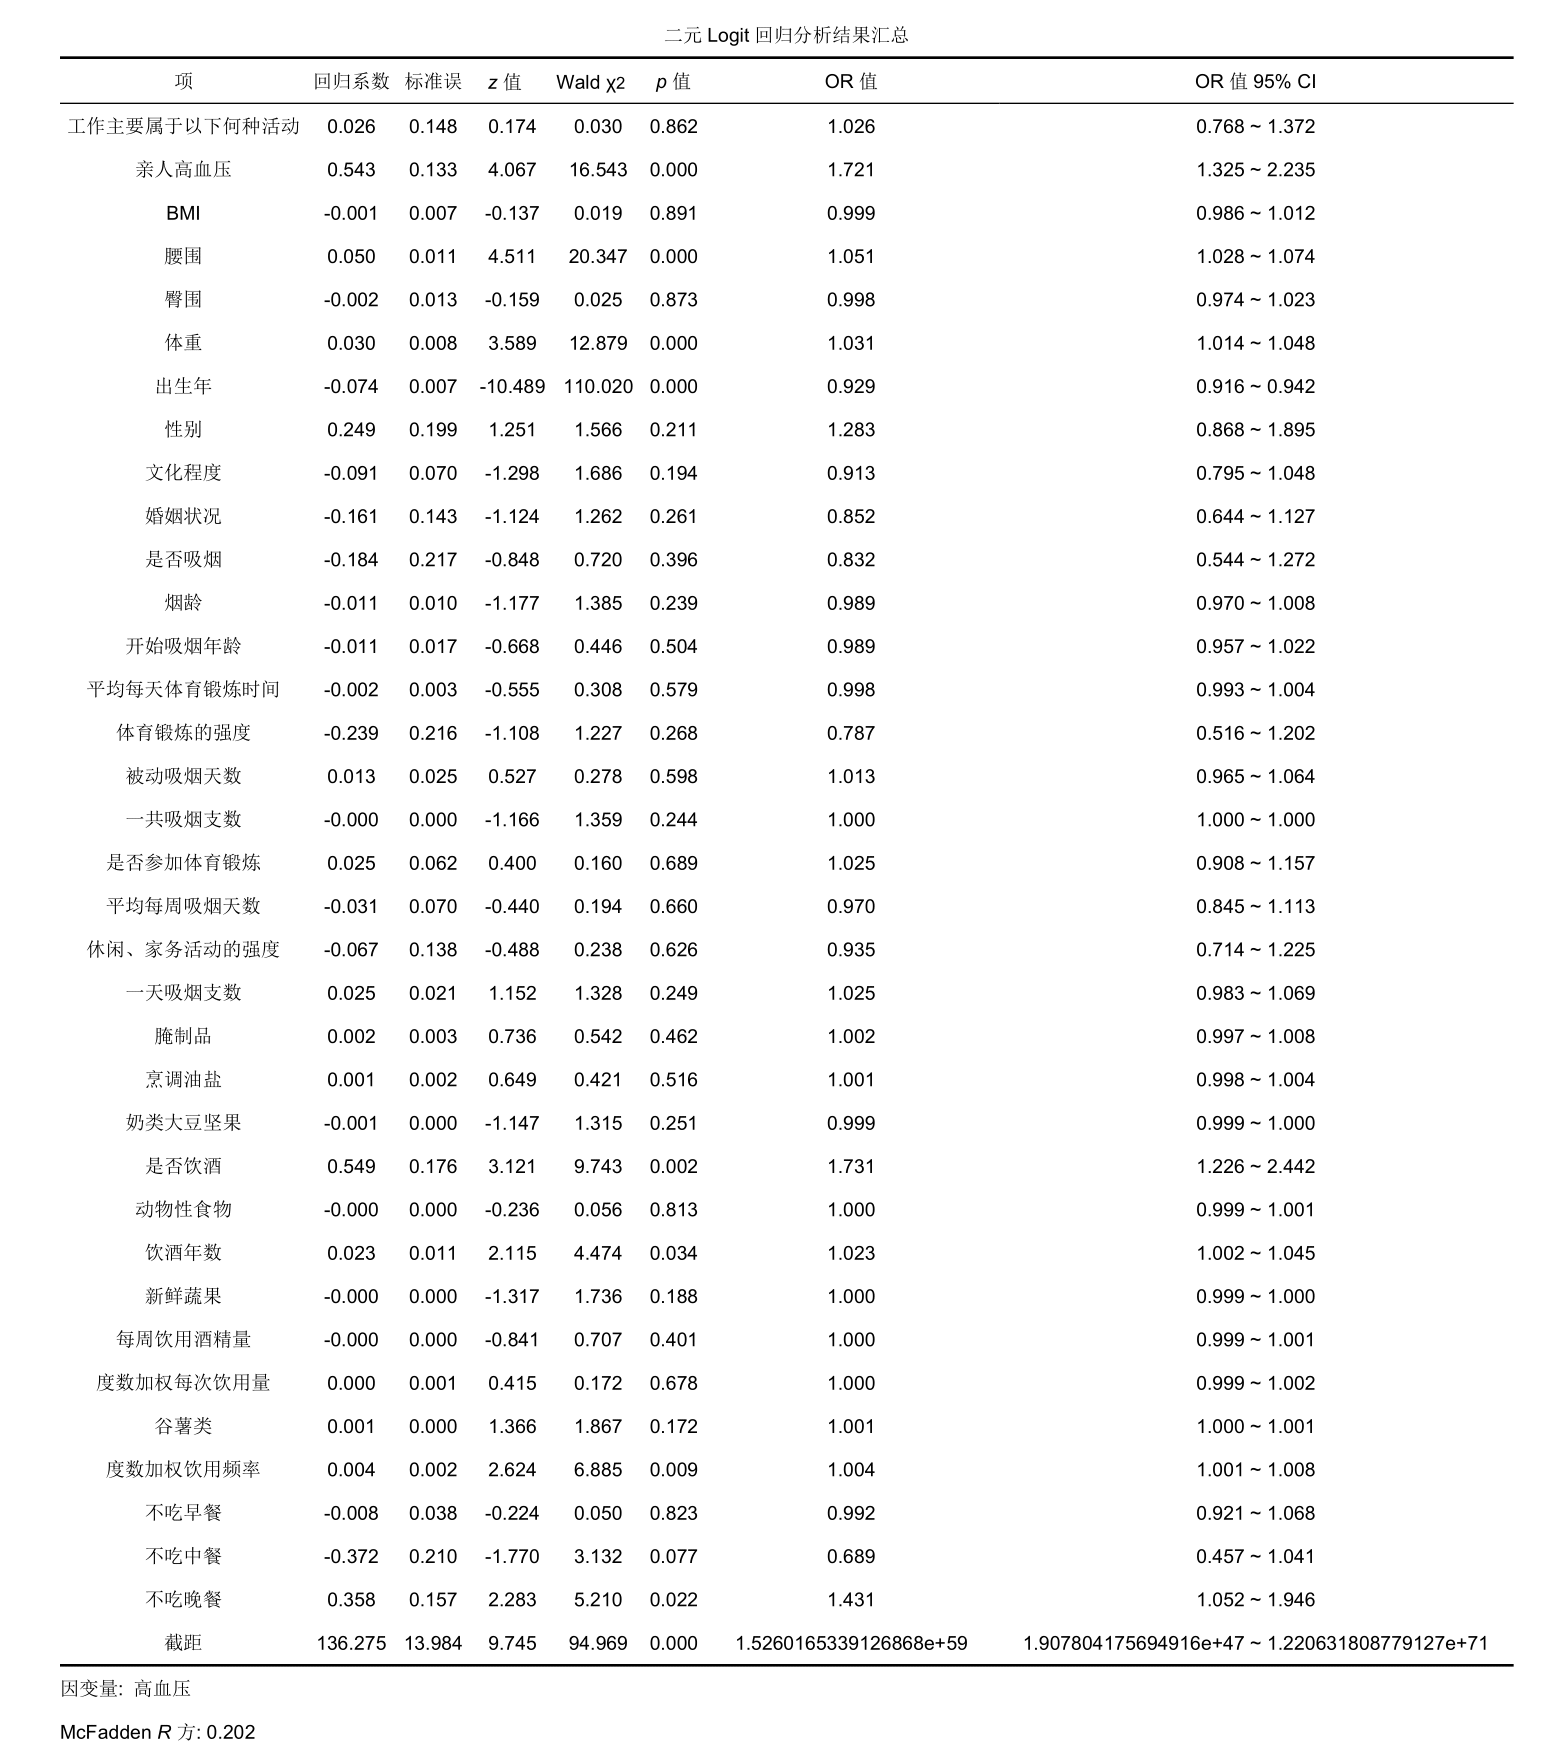
\includegraphics[scale=0.78]{logit1.png}
    \caption{高血压数据第一次logistic回归结果}
\end{figure}
\newpage
3.2糖尿病第一次logistic回归结果
\begin{figure}[H]
    \centering
    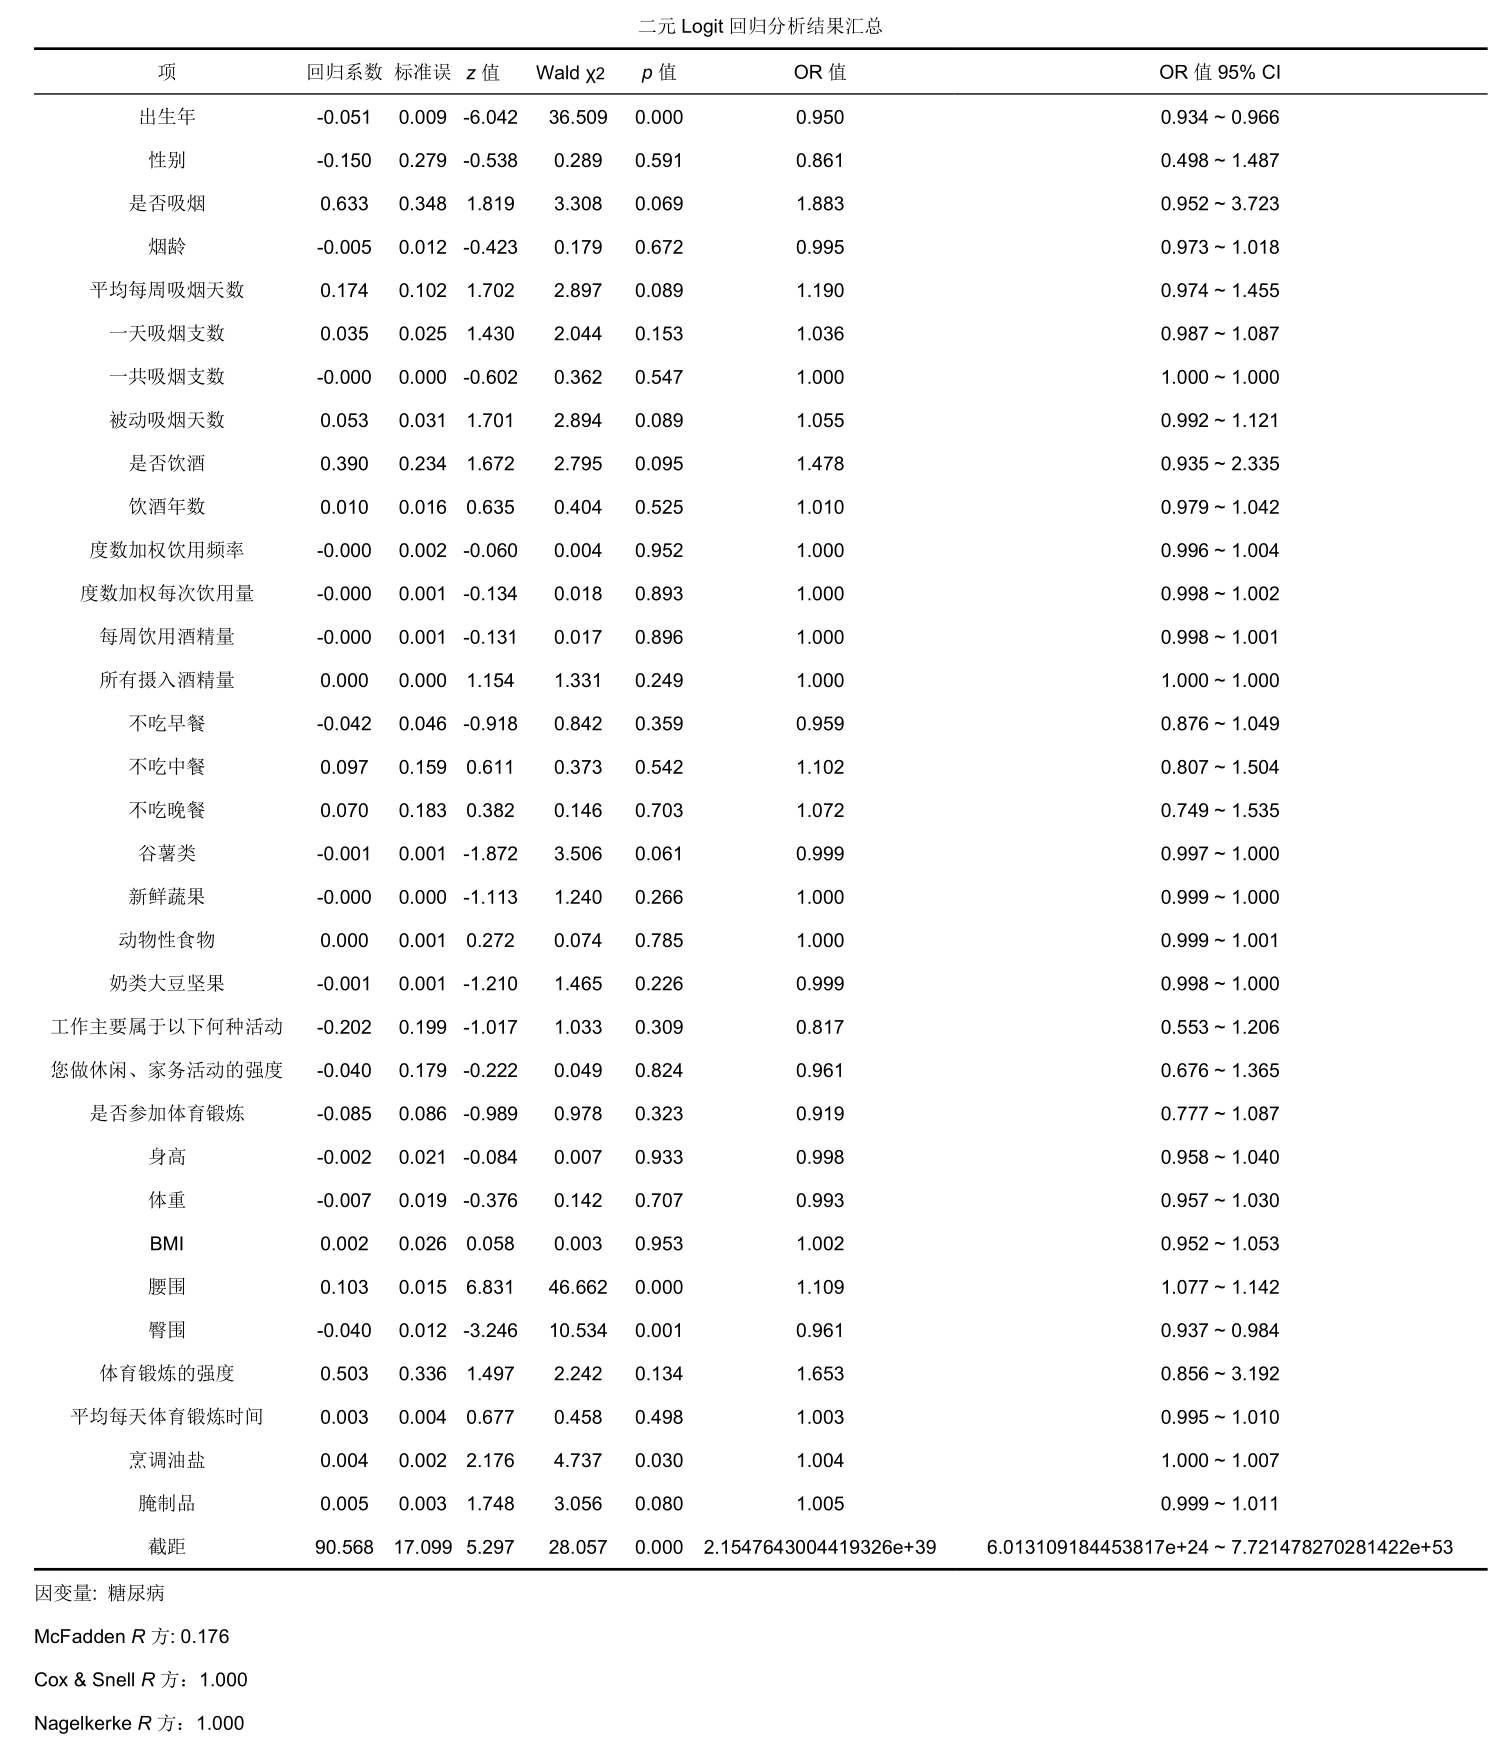
\includegraphics[scale=0.78]{logit3.png}
    \caption{糖尿病数据第一次logistic回归结果}
\end{figure}

\newpage
$(F{[x]},a)$ \\
$\aleph 0 $\\

$\varphi  \in \mathrm{Hom}\left((F{[x]},c),(K^m,J_m)\right), dim\varphi=dim(null(c^T\otimes I_m-I_c\otimes J_m))\geq \aleph 0$\\
$$
a^T\otimes I_m-I_a\otimes J_m=
\begin{pmatrix}
    a^T&-I_a&0&0&\cdots&0&0\\
    0&a^T&-I_a&0&\cdots&0&0\\
    0&0&a^T&-I_a&\cdots&0&0\\
    \vdots&\vdots&\vdots&\ddots&\ddots&\vdots&\vdots\\
    0&0&0&0&\ddots&-I_a&0\\
    0&0&0&0&\cdots&a^T&-I_a\\
    0&0&0&0&\cdots&0&a^T\\
\end{pmatrix}_{m\aleph 0 \times m\aleph 0 }
$$
$a^T$\\
$\aleph 0 \times \aleph 0$\\
$\exists\, n\in N, \;st\;a^n\equiv 0$\\
$J_c$\\
$J_a^n\equiv 0$
$$
J_cD=
\left(
    \begin{array}{cccccc :ccc}
    J_{k_1}&0&0&\cdots&0&\cdots&0&\cdots&0\\
    0&J_{k_2}&0&\cdots&0&\cdots&0&\cdots&0\\
    0&0&J_{k_3}&\cdots&0&\cdots&0&\cdots&0\\
    \vdots&\vdots&\vdots&\ddots&\vdots&\ddots&\vdots&\ddots&\vdots\\
    0&0&0&\cdots&J_{k_n}&\cdots&0&\cdots&0\\
    \vdots&\vdots&\vdots&\ddots&\vdots&\ddots&\vdots&\ddots&\vdots\\\hdashline
    0&0&0&\cdots&0&\cdots&0&\cdots&0\\
    \vdots&\vdots&\vdots&\ddots&\vdots&\ddots&\vdots&\ddots&\vdots\\
    0&0&0&\cdots&0&\cdots&0&\cdots&0
    \end{array}
\right)_{\aleph 0 \times \aleph 0 }
$$
$0<k_1,k_2,\cdots,k_n\cdots \leq n$\\
$\mathrm{Nil}(C)$\\
$(C,c),(D,d),\; \varphi \in\mathrm{Hom}\left((C,c),(D,d)\right)$
\\
$dim\varphi=dim(null(J_c))=\aleph 0$\\
$\forall x\in C,\exists n_x\in N,\;st\;c^{n_x}x\equiv 0$

$dim(F[x])=\aleph 0$

$a:F[x]\longrightarrow F[x],\;f(x)\longmapsto f^{(k)}(x)\quad(\forall k\in \mathrm{N_+})\quad;\quad \forall f\in F[x],\;\exists n_f\in N_+ \;st\;a^{n_f}f\equiv 0$

$J_c^{n_f}\equiv 0$

$J_{\aleph 0}$

$(k<\infty)$

$J_k$

$0_{\aleph 0}$

$0_k$

$J_{\aleph 0-1}$


\end{document}


